\documentclass[
BCOR 0.7cm,							% Bindekorrektur, bspw. 1 cm
11pt										% Schriftgroesse
]{scrbook}


\newif\ifpdf
\ifx\pdfoutput\undefined
	\pdffalse              	%normales LaTeX wird ausgef�hrt
\else
	\pdfoutput=1           
	\pdftrue               	%pdfLaTeX wird ausgef�hrt
\fi

\ifpdf
	%\usepackage{ae}        % Benutzen Sie nur
	%\usepackage{zefonts}  	% eines dieser Pakete
\else
	%%Normales LaTeX - keine speziellen Fontpackages notwendig
\fi

\ifpdf %%Einbindung von Grafiken mittels \includegraphics{datei}
	\usepackage[pdftex]{graphicx} %%Grafiken in pdfLaTeX
\else
	\usepackage[dvips]{graphicx} %%Grafiken und normales LaTeX
\fi


\ifpdf
	\pdfinfo
	{
    /Author (Manfred Kindl)                                
    /Title (CIS)     
    /Subject (CIS - Handbook)                                    
    /Keywords (CIS FH-Complete)	
  }
\else			
\fi

\usepackage{listings} \lstset{numbers=left, numberstyle=\tiny, numbersep=5pt}
\lstset{language=tex} 


\usepackage[pdftex,colorlinks=true,urlcolor=blue,linkcolor=blue]{hyperref}
\usepackage[ngerman]{babel}		%Deutsche Worttrennung	
\usepackage[T1]{fontenc}    % T1-Kodierung damit Umlaute richtig dargestellt werden
\usepackage[left]{eurosym}   %Paket f�rs Eurosymbol
\usepackage[latin9]{inputenc} % latin9 Encoding
\usepackage{makeidx} % Stichwortverzeichnis erstellen aus \index{} Eintr�gen
\usepackage{float}
\usepackage[small,bf]{caption}
\usepackage{fancyhdr} % Paket zur Manipulation von Kopf und Fusszeile
\usepackage{amssymb,amsmath}
\usepackage{color}
\usepackage{hyperref} % Paket zum formatieren der Hyperlinks
\hypersetup{colorlinks=false} % Formatiert die internen Links nicht. Optionen siehe unter: http://en.wikibooks.org/wiki/LaTeX/Hyperlinks#Customization

\addtokomafont{chapter}{\color[rgb]{0.0,0.376,0.584}}
\addtokomafont{section}{\color[rgb]{0.0,0.376,0.584}}
\addtokomafont{subsection}{\color[rgb]{0.0,0.376,0.584}}


\renewcommand{\rmdefault}{phv} % Arial
\renewcommand{\sfdefault}{phv} % Arial


\makeindex

\graphicspath{{../../../images/}}

\setlength{\tolerance}{2000}
\setlength{\parindent}{0pt}
\setlength{\parskip}{1ex plus 0.5ex minus 0.2ex}
\addtolength{\textheight}{2cm}
\addtolength{\headheight}{2pt}
\setlength{\captionmargin}{20pt}
\floatstyle{plain}
\floatname{example}{Example}

\newfloat{example}{hbtp}{loe}[chapter]
\floatplacement{figure}{hbtp}
\floatplacement{table}{htbp}

\newcommand{\dollar}{\char36}
\renewcommand{\labelitemi}{
\includegraphics[width=5pt]{blacksquare}}
\renewcommand{\labelitemii}{--}
%\renewcommand*{\chapterformat}{\textcolor{red}}

\newenvironment{info}[1]{
    %\hspace{-10mm}
     \framebox[\textwidth][l]{
        \begin{minipage}{1,3cm}
        
\includegraphics[width=1cm]{icon_info}
        \end{minipage}
        \begin{minipage}{12cm}
        #1
        \end{minipage}
    }
}

\newenvironment{achtung}[1]{
    %\hspace{-10mm}
     \framebox[\textwidth][l]{
        \begin{minipage}{1,3cm}
        
\includegraphics[width=1cm]{icon_achtung}
        \end{minipage}
        \begin{minipage}{12cm}
        #1
        \end{minipage}
    }    
}

\newenvironment{halt}[1]{
    %\hspace{-10mm}
     \framebox[\textwidth][l]{
        \begin{minipage}{1,3cm}
        
\includegraphics[width=1cm]{icon_halt}
        \end{minipage}
        \begin{minipage}{12cm}
        #1
        \end{minipage}
    }
}

\newenvironment{idee}[1] {
    %\hspace{-10mm}
     \framebox[\textwidth][l]{
        \begin{minipage}{1,3cm}
        
\includegraphics[width=1cm]{icon_idee}
        \end{minipage}
        \begin{minipage}{12cm}
        #1
        \end{minipage}
    }
}


\setlength{\unitlength}{1mm}

\newenvironment{markier}[5]{
    
    \thicklines \put(#2,#3){\vector(#4,#5){5}} \thinlines
    \put(#2,#3){\circle*{5}}
    \put(#2,#3){\textcolor{black}{\circle{5}}\makebox(-10,0){\textcolor{white}{#1}}}


}


\hyphenation{gleich-zeitig para-meter}


\begin{document}

\ifpdf
	\DeclareGraphicsExtensions{.pdf,.jpg,.png}
\else
	\DeclareGraphicsExtensions{.eps}
\fi

\pagestyle{fancyplain}

%% Titelseite einbinden %%%%%%%%%%%%%%%%%%%%%%%%%%%%%%%%%%%%%%%%%%%%%

%
% Titelseite, Abstrakt, Danksagung und Inhaltsverzeichnis
%
%% eigene Titelseitengestaltung %%%%%%%%%%%%%%%%%%%%%%%%%%%%%%%%%%%%%%%    

\begin{titlepage}
\begin{center}

\vfill 
\includegraphics[width=1\textwidth]{fhcomplete}
\vspace*{20mm}
\vfill 
\includegraphics[width=100mm]{cis}
\vspace*{10mm} 

\huge Handbook\\

	
\large \vfill UAS Technikum Wien\\

Vienna, \today
\end{center}
\end{titlepage}

\tableofcontents			% Inhaltsverzeichnis
\frontmatter					% Vorspann (z.B. r�mische Seitenzahlen)
%\chapter{Einleitung}
%\info{Alle im Handbuch gezeigten Abbildungen wurden mit Daten aus der Entwicklungsdatenbank zur besseren Veranschaulichung der Abl�ufe erzeugt. Die Inhalte der Listen, wie etwa Betr�ge oder Zugriffsrechte, sind frei erfunden und haben keinen Bezug zu den Daten des Echtsystems.}
\mainmatter						% Hauptteil

%% Kapitel Anfang %%%%%%%%%%%%%%%%%%%%%%%%%%%%%%%%%%%%%%%%%%%%%%%%%

\chapter{Definitions, Features, and Abbreviations Used}
\label{Kapitel Begriffe} 

	\minisec{Unit}
...see teaching unit.
	
	\minisec{Department}
...see Institute.

	\minisec{Institute}
An institute is the entity responsible for allocating lecturers for the individual degree programs and subjects.
An example is the "`Languages"' Institute, which is responsible for all language-related subjects. (English, French, Japanese,...)

	{\minisec{Schedule Conflicts}
TEMPUS\raisebox{1ex}{\tiny\copyright} 2.0 checks the availability of lecturers, students and rooms as well as the times lecturers have marked as unavailable and reservations when making entries or changes to the teaching schedule. Should there be a scheduling conflict with one of the three schedules, an error message will appear and the action will be cancelled.
However, a conflict can be forced by disabling the conflict check in the "'Settings"' menu. The conflict check should always be enabled again afterwards, as otherwise this could easily lead to errors in the scheduling. (see chapter \ref{Kapitel Kollisionen})

	\minisec{KW...Calendar Week}
The year consists of at least 52 numbered calendar weeks (CW). According to DIN 1355 / ISO 8601, the first week of the year is the week in which at least four days fall in the new year. 

	\minisec{University Council}
The University Council consists of all the program directors, teacher representatives, heads of the departments and students, and is responsible for making all important strategic decisions for the UAS Technikum Wien.
	
	\minisec{LE...Teaching Unit}
The teaching unit contains all the essential, variable data needed to carry out the schedule planning. The data in the teaching units is used specifically for planning the teaching schedule and also as a source for the CIS page. Teaching assignments are also created based on this data. 

The teaching unit brings lecturers, students, subjects, etc. together and must be revised each semester.

See chapter \ref{Kapitel Lehreinheiten} for a detailed description.

For comparison, see "'LV...Course"'

	\minisec{Teaching Unit\_ID}
The teaching unit\_ID is a unique internal number that is assigned to each teaching unit.
Most tables in the database are linked to the teaching unit\_ID

	\minisec{Subject}
A subject determines the content of a teaching unit. (e.g., mathematics)

It defines the department responsible, the color (which is displayed in the teaching schedule), and the language of instruction. A subject is created for each degree program and each corresponding semester. The abbreviation for the subject is displayed together with the course type at the top of the teaching schedule. 
The course type for the classroom instruction (exercise, lecture, ILV,...) is, however, not defined here.

	{\minisec{Course Type}
The course type describes the subject in more detail in that it specifies the type of teaching that will take place. 

A course type can be a lecture (-VO) for example. This describes frontal teaching without independent practice. 

Other examples include exercise (-UE), integrative course (-ILV), lab sessions (-LAB) or tutorials (-TUT)

	\minisec{Teaching Schedule (=Timetable)}
The teaching schedule is the surface on which the teaching units are graphically displayed in color with the lecturers, the teaching groups and the rooms. 

It is possible to browse through the rooms and course weeks in the teaching schedule and it can also be exported from here for various other applications.

	\minisec{Teaching Group}
The teaching group refers to the organization of students into degree program, semester, divisions and groups. 

It serves to organize and divide larger numbers of students to create smaller groups for a better overview. 

An example at the UAS Technikum Wien would be: BEL-2A1. (Bachelor's Degree Program Electronics, 2nd Semester, Division A, Group 1) 

	\minisec{LFVT...Degree Program Course Schedule}
The degree program course schedule is the complete list of all teaching units that are to be planned for a semester of a degree program.

	\minisec{LV...Course}
A course is understood in the overall system the same as it is in the application of the degree program. It contains the basic master data. In contrast to the teaching unit, the course contains data that generally remain unchanged from year to year. It forms the basic foundation upon which all other tables are built.\\
The course is always seen from the perspective of a degree program or from the perspective of the student. The title of the course can be found on the transcripts and in the Teaching section on the CIS page. The course is not to be confused with the subject or the teaching unit (see individual definitions).\\
Courses that have been used once can no longer be removed but only disabled because otherwise the student grades for the course would be lost.

Attributes of the course are, for example, the abbreviation, the degree program, the semester in which it is taught, the language, the ECTS credits or the semester hours.

	\minisec{Module, Special Groups}
In addition to the regular teaching groups, there are modules and special groups which may contain different students.
It is thus possible to create groups of students from different teaching groups within a semester, or even from different semesters or degree programs. However, since special groups make it significantly more difficult to check for schedule conflicts and produce a teaching schedule without errors, special groups should be avoided as far as possible.

	\minisec{Infotip}
An infotip appears when the user holds the mouse over an element for a short time without clicking.

	\minisec{Room Type}
The attribute "'Room Type"' is used to summarize the various classrooms.
For example, a room type might be "'seminar room"'. This combines any number of single rooms into a whole.
The attribute is mainly used to obtain a clear number of suggested rooms for a teaching unit when planning the teaching schedule.

	\minisec{Reservation}
The teaching plan allows lecturers and staff to reserve a room in order to ensure they have a room available in the medium term and to keep the room from being used for the teaching schedule or by other teachers and staff.
It is only possible to reserve a room within a predefined time frame. Any reservation that has been made generally has precedence over regular teaching.

In practice, this may sometimes prove extremely inconvenient. Often external events, guest lectures, parties and graduation ceremonies are the reason for inconvenient changes to the room allocations. However, these irregular events are an important part of the University's day to day business, so it is not likely that a more convenient solution will be found other than giving priority to such events.

	\minisec{Semester (Year)}
A semester (from Latin: sex=six; mensis=month) is half of an academic year at a university. This also includes the semester break (= time in which there are no lessons).
As a rule, odd semesters (1,3,5,...) are in the winter semester (from September to February) and even semesters (2,4,6,...) are in the summer semester (from March to August) 

	\minisec{Special Groups}
...see Modules

	\minisec{Degree Program}
A degree program is the learning content offered at a university that culminates in the award of an academic degree. 

The curriculum of a degree program is defined by the study regulations and the examination results and the completion of the degree program are defined by the examination regulations. 

A degree program is concluded with the awarding of an academic degree such as a Bachelor's, or Master's degree.

	\minisec{Study Semester}
The study semester is a unique designation for a semester and a calendar year.
Accordingly, "'WS2007"' is the winter semester in 2007.

	\minisec{Blocking of Teaching Units}
The blocking of teaching units indicates how many units should be scheduled at a time (i.e. in direct succession). Since a single unit (for units of 45 minutes) is often inadequate, the blocking of teaching units will in most cases be at least "'2"'.

	\minisec{Timetable}
...see Teaching Schedule

	\minisec{UNR...Teaching Unit Number}
The teaching unit number is a sequential number that is automatically generated by the system and is relevant mainly for background processes. Normally, the UNR is the same as the teaching unit\_ID. 
It is important to note that the conflict check for the teaching schedule is based on the UNR. Teaching units with the same UNR can therefore be scheduled parallel to each other without causing an error.

	\minisec{Unit}
A day can be divided into any desired number of units with a starting and an ending time. However, the starting times may not overlap.
For example, at the UAS Technikum Wien, the day is divided into 16 units of 45 minutes each starting at 8:00 a.m.

	\minisec{Weekly Rhythm}
If a course is held at regular intervals throughout the semester, the interval can be specified in the attribute "'Weekly Rhythm"'.
A weekly rhythm of "'2"' therefore means that the course should take place every 2 weeks.

	\minisec{Unavailable Time}
"'Unavailable Time"' is an extension of the "'Preferred Teaching Time"' feature designed to obtain detailed information about the availability of a lecturer.
It is thus possible for the lecturer to mark an unlimited amount of specific dates as unavailable (for example, due to conferences, stays abroad, vacation or training). An unavailable time is highlighted in the LV-Plan in dark-red and an error will occur should anything be scheduled for this time. (see chapter \ref{Kapitel Kollisionen})

	\minisec{Preferred Teaching Time}
In their profile, each lecturer is able enter their preferred teaching time based on a normal week grid. The lecturer can assign values from -2 to +2 for every day and every unit in a week to indicate their availability. This pattern is then applied for all the weeks of a semester.
The preferred teaching times should be chosen according to the fair play principle, so that at least three times as many teaching units are assigned a positive value as are to be taught according to the teaching assignment.

\begin{tabular}{rll}
+2&...&I would like to teach at this time\\
+1&...&I can teach at this time\\
-1&...&I can only teach at this time in emergencies\\
-2&...&I can not teach at this time\\
\end{tabular}

The values are shown in the background according to a color system (from red to green). The default is +1. 

Practice shows that the lecturers often do not take advantage of this feature or have such limited flexibility that it is not possible to plan a teaching schedule without problems. In some cases, even fewer teaching units are assigned a positive value than the lecturer is actually supposed to teach each week.
Furthermore, the preferred teaching times are rarely updated, which in turn leads to subsequent changes.
For this reason a disciplined use of the preferred teaching times is an essential basis for effectively planning the teaching schedule.

The TEMPUS\raisebox{1ex}{\tiny\copyright} program indicates the preferred teaching time with a background color when selecting a lecturer or setting a teaching unit.

\begin{figure}
	\centering
	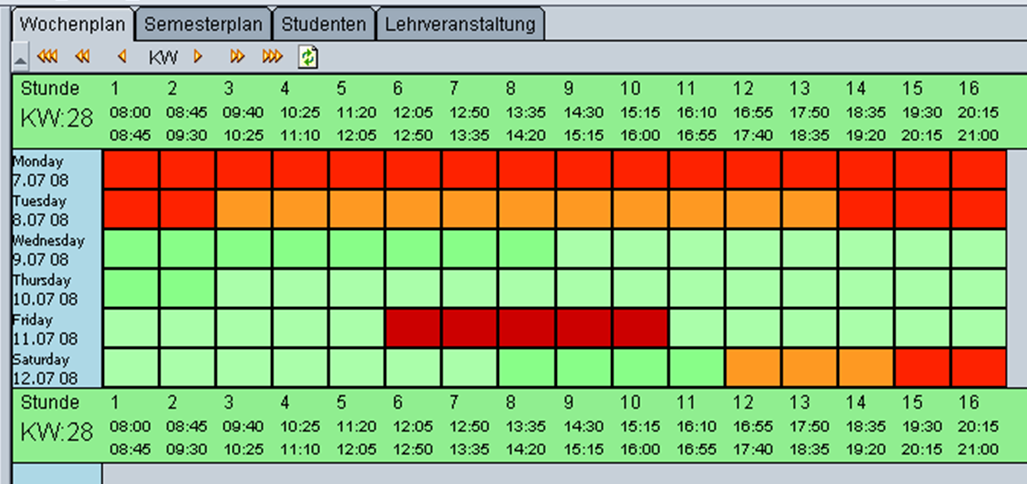
\includegraphics[width=0.8\textwidth]{Tempus_Beispiel_Zeitwunsch}
	\caption{Example of a preferred teaching time with all four values and a time on Friday marked as unavailable (dark red)}
	\label{Zeitwunsch}
\end{figure}

\chapter{General}
\section{Overview}

The Campus Information System is the central web interface for students and staff. Various services are available here.
You can read the latest news, access information about the teaching and courses offered, look up teaching schedules and much more. 

\begin{figure}
	\centering
	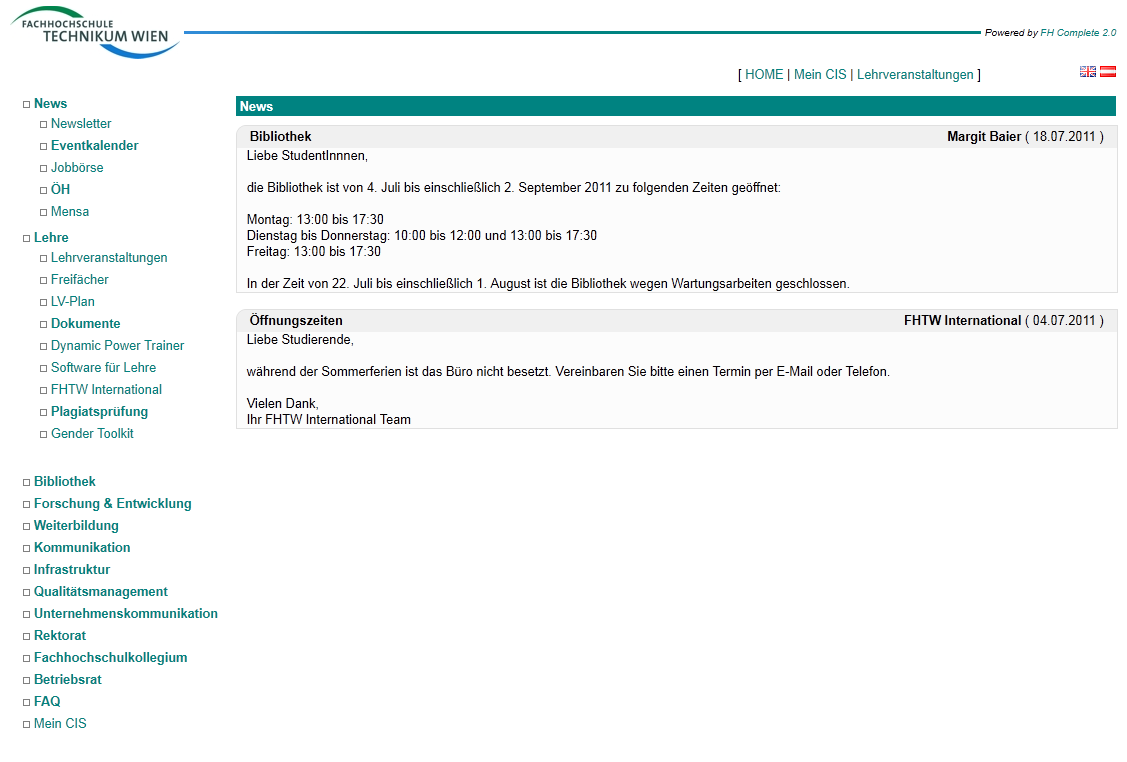
\includegraphics[width=0.70\textwidth]{CIS_Startseite.png}
	\caption{CIS HOME}
	\label{CIS_startseite}
\end{figure}

\section{Main Menu Sections}

	\minisec{News}
The CIS offers various news pages (also called Pinboard in the Course News section). The HOME page shows the view for "'General News"'. In addition, there are pages for each organizational unit (Degree Program, Institute,...). These are displayed on the appropriate sub-page together with the general news.
For the guidelines on managing news please see \ref{richtlinien_newseintraege}

The "'News"' section of the CIS also includes links to other external news and information platforms.

	\minisec{Teaching}
The Teaching section contains all the information and documents necessary for teaching, such as information about courses, attendance lists, grade lists, participant lists, mail groups, semester plan and the student upload tool to make carrying out exercises easier.

Furthermore, in this section you can also register for electives and find tools and information to help you with your teaching.
For more details, please see chapter \ref{lehre}.

	\minisec{Library}
Here you will find information about the library, research links, links to electronic media and external literature databases as well as the OPUS publication database.

	\minisec{Research \& Development}
In this section you will find information about ongoing projects as well as documents and procedures for conducting research projects.

	\minisec{In-service Training}
Here you can learn about which internal and external in-service training programs are currently being offered.

	\minisec{Communication}
Here you can view your contacts, webmail, UAS Technikum Wien mailing lists or search for a specific person.

	\minisec{Infrastructure}
The Infrastructure section contains the most important information about the technical and logistical infrastructure of the university:
Instructions and tools for connecting to the LAN and Wi-Fi networks, a free antivirus program, information about the media equipment available, maps, as well as regulations.

	\minisec{Quality Management}
Here you will find all the documents and processes relevant for studying at the UAS Technikum Wien, documents concerning the general organization of the UAS, as well as the relevant document templates.

	\minisec{Corporate Communications}
In this section you will find the UAS Technikum Wien company logo, corporate identity handbooks and an event guideline available for download.

	\minisec{Rector's Office}
Under "'Rector's Office"' you will find the UAS Technikum Wien mission statement, key figures, gender mainstreaming activities, university projects, awards and information on competitive tenders and grants.

	\minisec{University Council}
	In this section you will find a list of members and the rules of procedure for the Council of the UAS Technikum Wien, as well as the relevant documents.

	\minisec{Union Info}
News, information and important documents like internal agreements are available here.

	\minisec{FAQ}
The FAQ (frequently asked questions) section provides various instructions, solutions to common problems, handbooks, and a link to the archive.

	\minisec{My CIS}
In this section you will find all of your personal information as well as a number of administrative tools:
an overview of your profile data, your personal teaching schedule, preferred teaching times, the vacation tool (for staff), your courses (for lecturers) and tools for submitting Bachelor's and Master's theses.
\chapter{Notification System}
\label{kapitel_ampelsystem}

\section{General}

The notification system is a reminder and confirmation system which can be used for students, lecturers and staff.
When the user logs in, their open notifications will be displayed in the title bar as red or yellow traffic lights based on their urgency (see Figure \ref{ampel_icons}).
Administrators can create and manage new notifications.

\begin{figure}
	\centering
	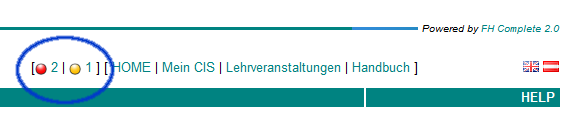
\includegraphics[width=0.70\textwidth]{CIS_Ampelsystem_Ampelicons.png}
	\caption{Notifications are displayed in the title bar as red or yellow traffic lights}
	\label{ampel_icons}
\end{figure}

Clicking on a traffic light will open an overview page where each notification can now be confirmed individually (see Figure \ref{ampel_uebersicht}).
A notification can be limited by the following parameters:
\begin{description}

	\item[Description:] Title and contents of the notification.
	\item[Target Group:] It is possible to define exactly who should receive a notification. Notifications can be displayed for defined groups of people (staff, students, ...) and/or individuals.
	\item[Deadline:] Specifies the date when a notification will be considered "`overdue"'. The traffic light will turn "`red"' on this date.
	\item[Lead Time (in days):] Specifies the date when a notification will be displayed as a "`yellow"' traffic light.
	\item[Expiration Time (in days):] Specifies when a notification will no longer be displayed. It does not matter if the notification has been confirmed or not.
\end{description}

\begin{figure}
	\centering
	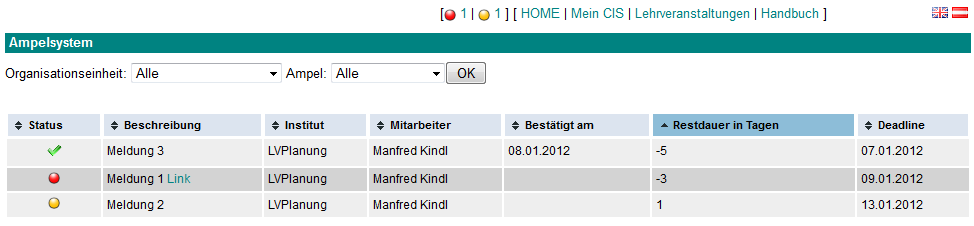
\includegraphics[width=1\textwidth]{CIS_Ampelsystem_Ampeluebersicht.png}
	\caption {Overview of the notification confirmation page}
	\label{ampel_uebersicht}
\end{figure}

\section{Overview of the Notifications}
\label{ampeluebersicht}

As can be seen in Figure \ref{ampel_uebersicht}, all the notifications are listed on the overview page. Notifications before the deadline are marked with a yellow traffic light, notifications that have exceeded the deadline are marked with a red traffic light and confirmed notifications are marked with a green check mark.
When a notification reaches the expiration date, it is no longer displayed (it does not matter whether it has been confirmed or not).

\subsection{Confirming a Notification}

To confirm a notification, click on "`Confirm"' in the last column. The notification will then be marked with a green check mark and will continue to be displayed as "`confirmed"' until the expiration date.

\section{Other}

You can sort the list by clicking the column headings.

\section{Overview of the Notifications for Heads of Departments}
\label{ampeluebersicht_leiterinnen}

If you have the appropriate user rights, you can view the status of all the notifications under "`My CIS -> Notification Overview"'.
This will provide you with an overview of exactly who has confirmed a notification or not.
You can filter the list according to organizational unit and/or traffic light descriptions and sort them by clicking the column headers.

The date on which a notification was confirmed can be seen in the column "`Confirmed on"'.
The column "`Remaining time in days"' displays how many days are remaining until the notification reaches the deadline, or in the case of negative numbers, the number of days by which the deadline has been exceeded.

\chapter{News}
\section{General}

The CIS offers various views for news (also called Pinboard in Course News section). The HOME page shows the view for "'General News"'. In addition, there are views for each organizational unit (degree program, department,...). Here the general news is displayed together with the specific news.

The right to publish news entries depends on the individual's user rights.
Lecturers may publish an unlimited number of news entries to the organizational units (e.g. degree programs) on the Pinboard.
The right to publish general news is issued on an individual basis by the system administration.

\section{Guidelines for News Entries}
\label{richtlinien_newseintraege}

The following guidelines must be observed when publishing news entries:
\minisec{General News}
General news should relate to the staff AND students and should also be directly related to our organization. Under no circumstances should this become an advertising platform for external events. 

\idee{General News is translated by the Infrastructure}

\minisec{OU News}
News in the organizational units is aimed at staff and students within the OU.
OU news is not automatically translated. However, the OU may translate news entries themselves.
See chapter \ref{uebersetzung_eines_neweintrags}

\section{Erstellung}

\subsection{How to Publish a General News Entry}
\label{allgemeinen_Newseintrag_erstellen}

The news administration for general news is located in the Infrastructure section under "'Administrative Tools"'.

\begin{figure}
	\centering
	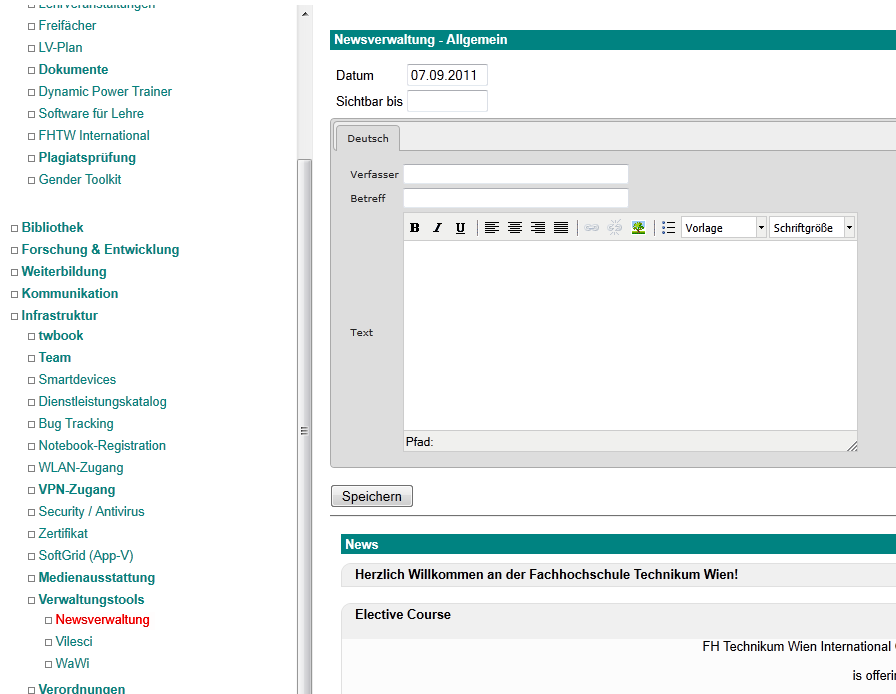
\includegraphics[width=0.70\textwidth]{CIS_Newsverwaltung_01.png}
	\caption{CIS General News Administration}
	\label{CIS_newsverwaltung01}
\end{figure}

		\begin{itemize}
			\item In the "'Date"' field, enter the date from which the news entry should be visible (default: today).
			\item In the field "'Visible to"', enter the date until when the news entry should be visible (max. 30 days). This field is optional, and if left blank the news entry will remain visible for 30 days.
			\item Enter the author name which will appear in the title line of the news entry.
			\item Enter a meaningful title for the article.
			\item Enter the text for the news entry and format it with the appropriate buttons. Holding your mouse over the different buttons will bring up an infotip that explains each button's function.
			You can adjust the size of the editing window by clicking and dragging the lower right corner of the window until it is the desired size.
			\item Finally, save the news entry by clicking on the "'Save"' button.
			\item You will find information on how to translate a news entry in the chapter \ref{uebersetzung_eines_neweintrags}.
		\end{itemize}
		
\subsection{How to Publish an OU Specific News Entry}
The news administration for the OU news can be found by clicking on the menu item "'Courses"' and then selecting the desired degree program.
Finally, click on "'Lecturer's Section"' and "'Pinboard Administration"'.

\begin{figure}
	\centering
	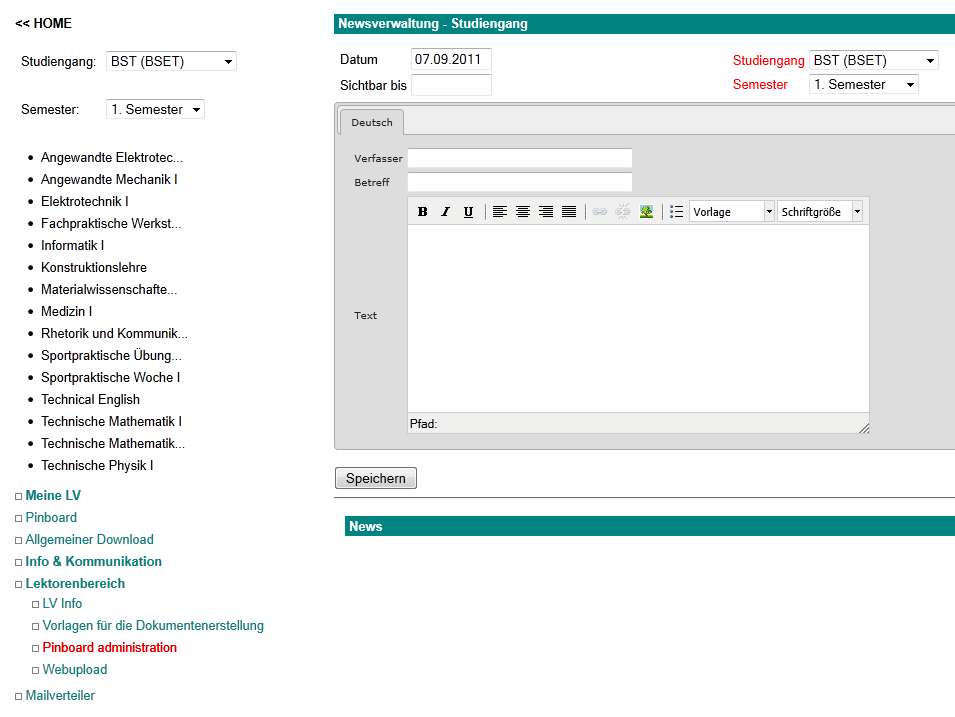
\includegraphics[width=0.70\textwidth]{CIS_Newsverwaltung_03.png}
	\caption{CIS News Administration for OU}
	\label{CIS_newsverwaltung03}
\end{figure}

Proceed with the news entry here the same as described in chapter \ref{allgemeinen_Newseintrag_erstellen} with the only difference being that you should select the relevant degree program and/or semester in the headline for those who should be able to view the news entry.

\subsection{How to Publish a Translation for a News Entry}
\label{uebersetzung_eines_neweintrags}
The Infrastructure will automatically send general news to the translator (does not apply for OU news) and will publish the translation as soon as it is available.
However, if you want to translate a news entry yourself or want to translate an OU news entry, please proceed as follows:
(also see chapter \ref{richtlinien_newseintraege} Guidelines for News Entries)
		\begin{itemize}
			\item After you have saved a news entry in the German language, a + symbol will appear next to the tab "'Deutsch"'.
				\begin{figure}
				\centering
				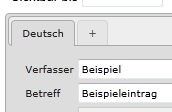
\includegraphics[width=0.30\textwidth]{CIS_Newsverwaltung_02.png}
				\end{figure}
			\item Click on "'+"' and select the desired language.
			\item Proceed with the news entry as described in Chapter \ref{allgemeinen_Newseintrag_erstellen}.
			\item Finally, save the news entry by clicking on the "'Save"' button.
		\end{itemize}
If the CIS page is now loaded in a different language, the news entry will now appear in the corresponding language if such a translation exists.
If there is no appropriate translation for a news entry in the German language, the news entry will be displayed in German.
\chapter{Teaching}
\label{lehre}
\section{General}

The "'Teaching"' section contains the most important links for your daily teaching.
Here you can view information about the courses, the teaching schedule, attendance lists, and semester schedules.

\section{Courses}
\label{lehre_lehrveranstaltungen}

On the "'Courses"' page you can first select the degree program and the semester you wish to view.

\begin{figure}
	\centering
	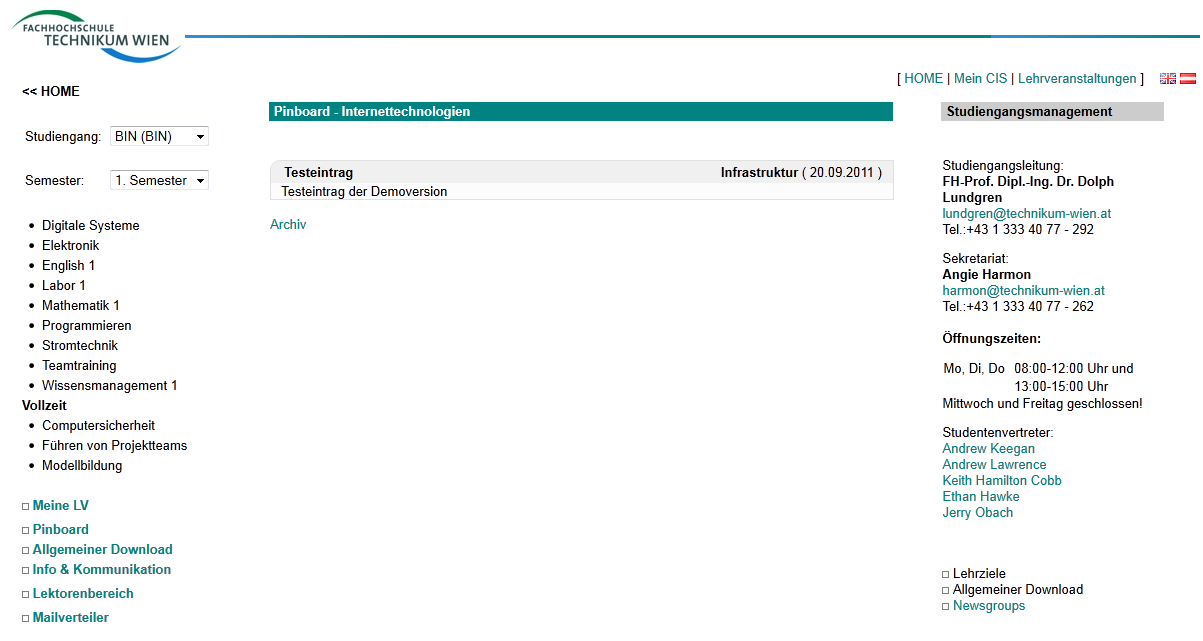
\includegraphics[width=0.70\textwidth]{CIS_Lehrveranstaltungen.png}
	\caption{CIS Courses}
	\label{CIS_lehrveranstaltungen}
\end{figure}

The news in the main window consists of the general news and specific news for the chosen degree program. If no specific news is available, only the general news entries will be displayed.

After selecting the desired degree program, all the active courses are listed.
If you select one of the courses, an overview will appear in the main window with all the tools and information available for this course. (see Fig. \ref{CIS_lehrveranstaltungen})

\begin{figure}
	\centering
	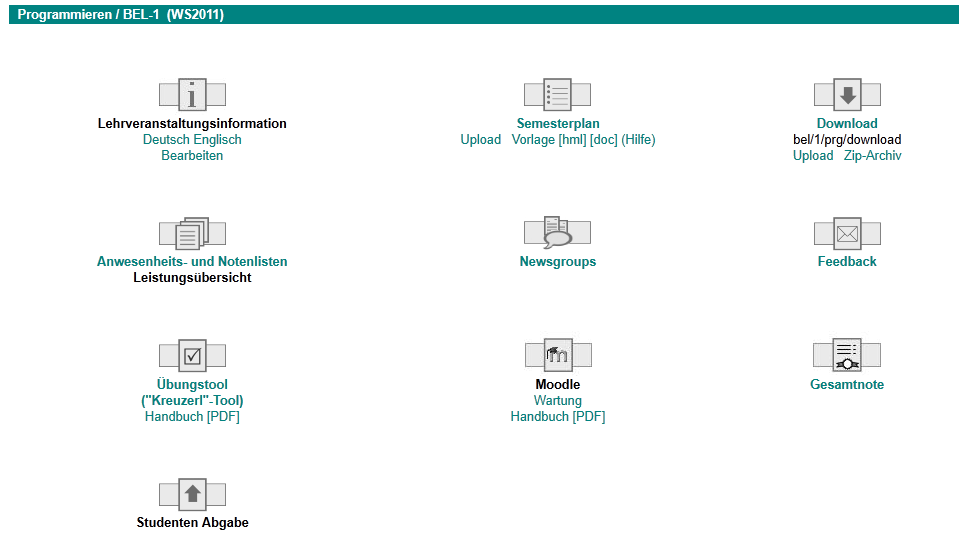
\includegraphics[width=0.70\textwidth]{CIS_Lehrveranstaltungen_Icons.png}
	\caption{CIS Courses Details}
	\label{CIS_lehrveranstaltungen}
\end{figure}

Here you can view the course information, semester plan, or the download area as well as generate attendance lists.
Furthermore, 3 tools are available to help you in your teaching: The activity tool, the student upload tool and the e-learning platform Moodle.

In the menu on the left you will also find the following sections:
\begin{description}
	\item [My Courses:] These are the courses in which you personally are a teacher or student.
	\item [Pinboard:] The news view with current information.
	\item [Global Download:] A link to the download area for the degree program.
	\item [Info \& Communication:] Here you will find a link to the teaching schedule, as well as to the webmail for you to manage your email.
	\item [Lecturer's Section:] Here you can edit the course information, upload documents and publish news entries if you possess the required user rights.
	\item [Mailing List:] Here you will find an overview of all the mailing lists at the UAS TECHNIKUM WIEN. By default, students are not granted access to large mailing lists.
\end{description}

\section{Electives}
\label{lehre_freifaecher}

Students can choose from any of the electives offered. The teacher is responsible for arranging the course times and dates.
The electives page is very similar to the courses page with only minor differences.
Here too it is possible to enter course information and semester plans as well as print out attendance lists.

On the left you will find the menu item "'Enrollment"' where you can mark all the desired electives and enroll for them by clicking on the "'Save"' button.
You can view the current enrollment status in the "'overview"'.

Withdrawal from an elective course is currently only possible by contacting the administrative assistant directly.

\section{Teaching Schedule}
\label{lehre_lvplan}

The teaching schedule is the UAS TECHNIKUM WIEN timetable.
You can select your personal schedule, the room schedule, the teaching schedule or the teaching group schedule.

\begin{figure}
	\centering
	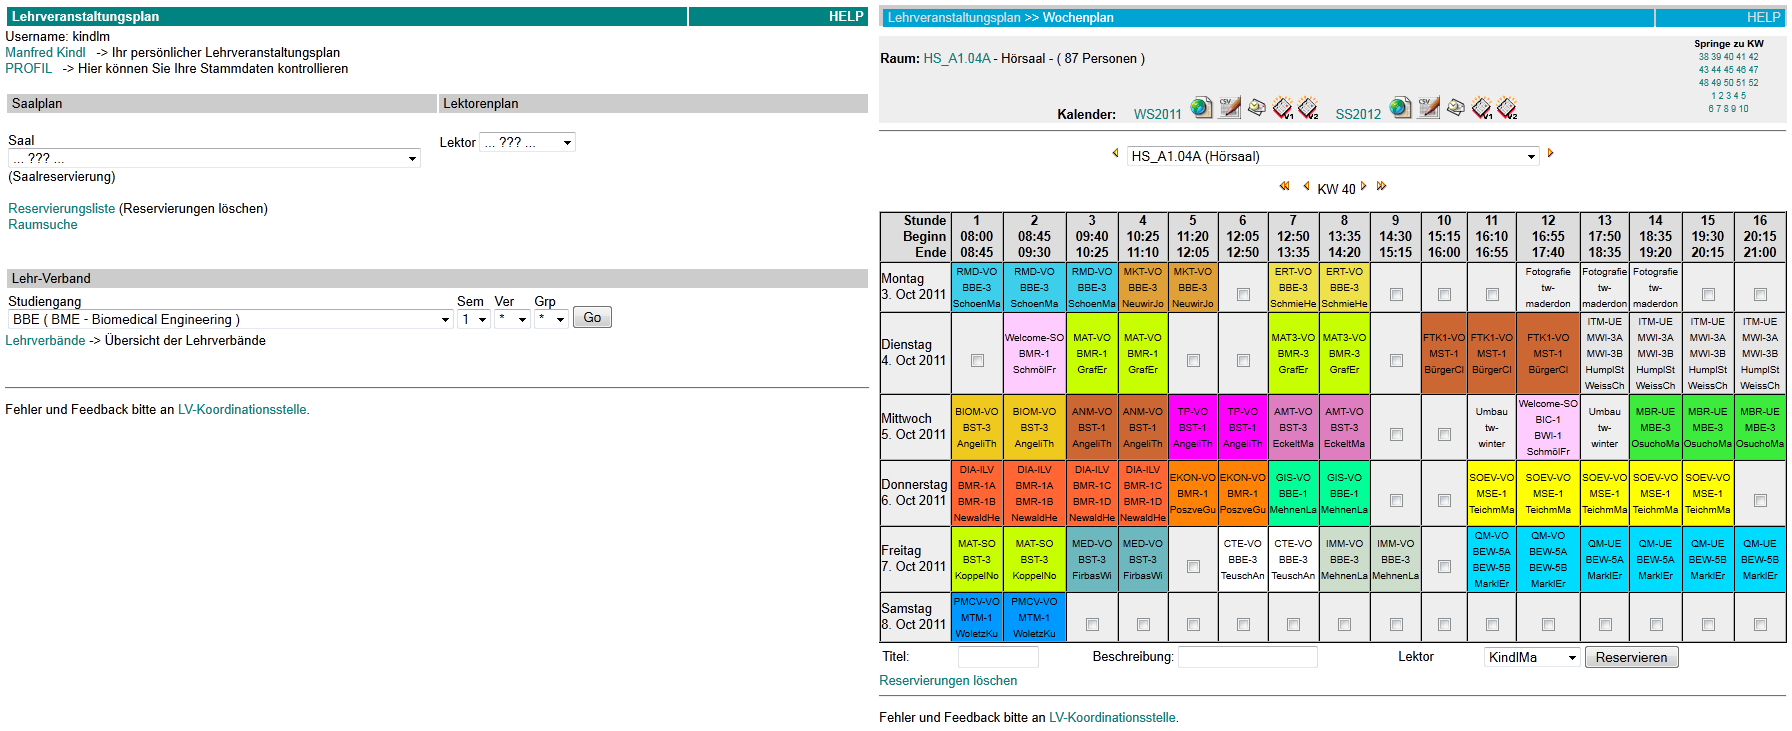
\includegraphics[width=1\textwidth]{CIS_Lvplan.png}
	\caption{CIS Teaching Schedule}
	\label{CIS_Teaching_Plan}
\end{figure}

\begin{description}
	\item [Personal Teaching Schedule:] Here you can view the teaching schedules that affect you personally. You only see the hours for your allocated group, any electives, if applicable, and your own reservations.
	\item [Room Schedule:] In this list you will find all the classrooms at the UAS TECHNIKUM WIEN and you can then view the schedule for each room. If you have the necessary rights, you can also make reservations using the room schedule.
	\item [Teaching Schedule:] allows you to view the timetable for a specific lecturer.
	\item [Teaching -Teaching Group:] Here you can view the schedule of each degree program optionally limited by semester, division and group.
\end{description}

\subsection{The Calendar View}

By clicking on the arrows here, you can move one week or four weeks forwards or backwards.
In the room schedule view you have an additional drop-down menu to scroll between the rooms.
If you click on an assigned unit, a details window will appear with additional information.

In addition, it is also possible to open the semester plan (overview with all the weeks arranged in a column) by clicking on WS20xx or SS20xx.

With the 5 icons next to each semester plan, you can export the teaching schedule to other clients (e.g. Outlook, Sunbird, Smartphone,...).

\subsection{Making Reservations}

You will require the appropriate rights (employees, lecturers, student representatives) to be able to reserve a room.
Select the location you want from the room schedule and mark the checkboxes for the units you want to reserve.
Afterwards, enter a title and a short description of the reason you wish to reserve the room.
Finally, click on the "'Reserve"' button.

\info{The reserved unit is visible only in the room schedule and in your personal schedule. If you want to make the reservation visible for a degree program, semester, or division, please contact the Scheduling Office}

\subsection{Deleting a Reservation}

You can view your reservations in the room schedule by clicking on "'Reservations List"' in the main menu or delete them by clicking on "'Delete Reservations"'.

\subsection{Room Information}

When you are in the room schedule, you can click the room name at the top left.
This will open a page where you can view detailed information about the equipment in the room, location information and pictures of the room.

\section{Documents}

Here you will find important and helpful documents related to everyday university life. Depending on your rights, you can access various folders and download files.

\section{Software for Teaching}

Here you will find software that can be used to help you in your teaching.

\begin{description}
	\item [Softgrid:] Is an environment-independent virtualization software with the application no longer being installed on the end device, but provided as a central application available any time. The local caching of the required applications allows you to take these applications "'with you"' and use them offline for up to 40 days. For installation details, see the "'Infrastructure"' section.
	\item [Dynamic Power Trainer:] Is a professional authoring software that you can use to create eLearning courses.
	\item [Moodle:] Is an object-oriented course management system and an open-source learning platform. The software offers possibilities for supporting collaborative teaching and learning methods.
\end{description}

\section{Plagiarism Check}

Both students and lecturers can submit their scientific work here for a plagiarism assessment by the external platform "'Ephorus"'.
\chapter{Vacation Management}
\label{urlaubsverwaltung}
\section{General}

The vacation management can be found under "'My CIS"' vacation tool.
The vacation tool is used as an extension of the unavailability times (see chapter \ref{zeitsperren_zeitwuensche}) in order to be able to register these times more easily and with a better overview.

\begin{itemize}
	\item The calculation period for vacation accruement is from September 1st of one year until August 31st of the following year.
	\item The administrative offices are responsible for calculating and managing the accrued vacation of all employees.
	\item The employee enters their desired vacation days in the vacation tool during the course of the year.
	\item The respective Head of Department or manager listed in the database will then be sent an email with a request for approval. Once they have been approved, vacation days can no longer be edited by the employee.
	\item The current accrued vacation is calculated from the effective date of August 31st. The Head of Department/manager will then enter the carry-over days into the system. The carry-over days, plus the number of currently accrued vacation days, minus the number of currently booked vacation days, equals the total accrued vacation from September 1st.
	\item The employee can view this calculation on the CIS page.
	\item If you are not assigned to an institute or are assigned to the incorrect institute, please contact Human Resources. 
\end{itemize}

\begin{figure}
	\centering
	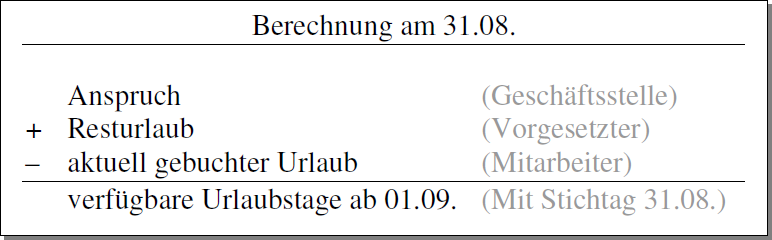
\includegraphics[width=0.70\textwidth]{CIS_Urlaubstool_Berechnung.png}
	\caption{Calculation of Accrued Vacation}
\end{figure}

\section{How to Use the Tool}

The vacation tool is accessed via the CIS page and serves as an extension to the user interface previously used for entering unavailable times. You can still enter and edit unavailable times here just as you did before.
We recommend using the following browsers: Mozilla Firefox or SeaMonkey.

\subsection{Booking a Vacation}

You can view your current accrued vacation and its calculation in the overview at the top left hand of the screen (see Fig. \ref{CIS_urlaubstool_eintragungen}). Clicking the help button will open a detailed description of the calculation.

\begin{figure}
	\centering
	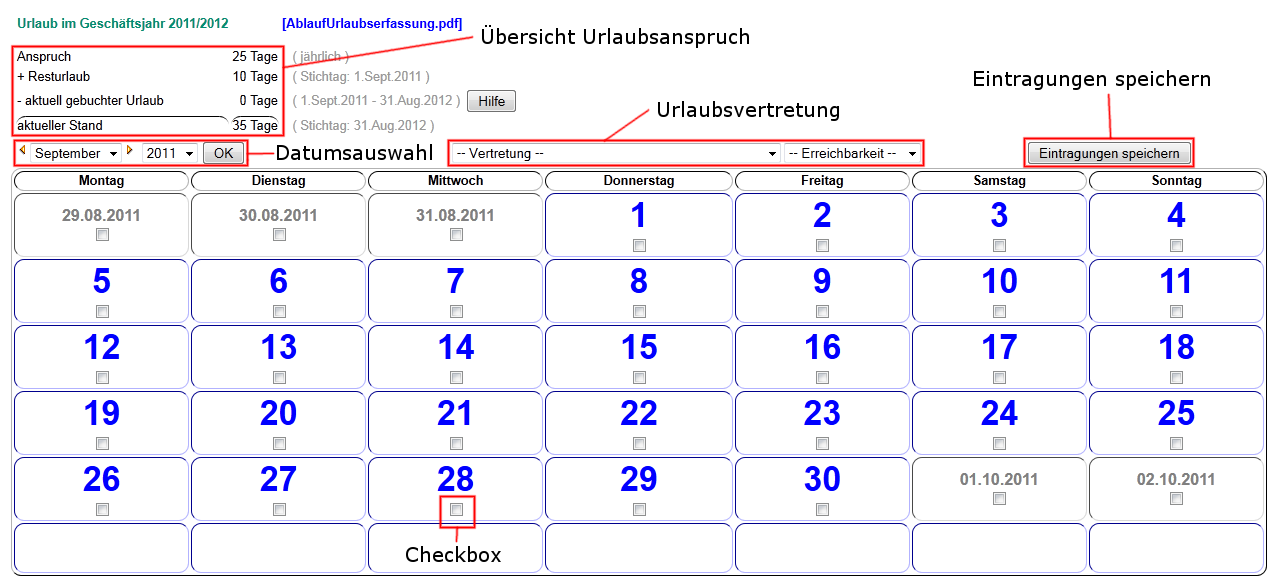
\includegraphics[width=1\textwidth]{CIS_Urlaubstool_Eintragungen.png}
	\caption{Save Vacation}
	\label{CIS_urlaubstool_eintragungen}
\end{figure}

Now select the month and year in which you want to book your vacation. You can select the year and month directly from the drop-down menus and \textbf{by pressing the OK button}, or by scrolling through the calendar with the yellow arrows.

You will see checkboxes underneath each weekday that can be selected or deselected with a simple click of your mouse.  Use these checkboxes to select the days you want to have free for your vacation.

\achtung{National holidays are not currently displayed in the calendar! Please check to ensure there are no national holidays during the time you have selected for your vacation.}

Now use the drop down menus to select your substitute and to indicate how you can be reached during your vacation. 
If you leave your contact information blank, your status will automatically be saved as "'Can not be reached!"'. Now press \textbf{Save Vacation}. 

The vacation time you have booked will now be highlighted in the calendar in light green. At the same time, an email will be sent to your manager with your vacation request and this is also confirmed by a red info text displayed below the calendar.

\info{If there is no manager assigned in the database, this will also be indicated in the info text. Should this be the case, please contact Human Resources.}

If you hold the mouse over a booked vacation (over the number), an infotip will appear with the substitute and information on how you can be reached.

\begin{figure}
	\centering
	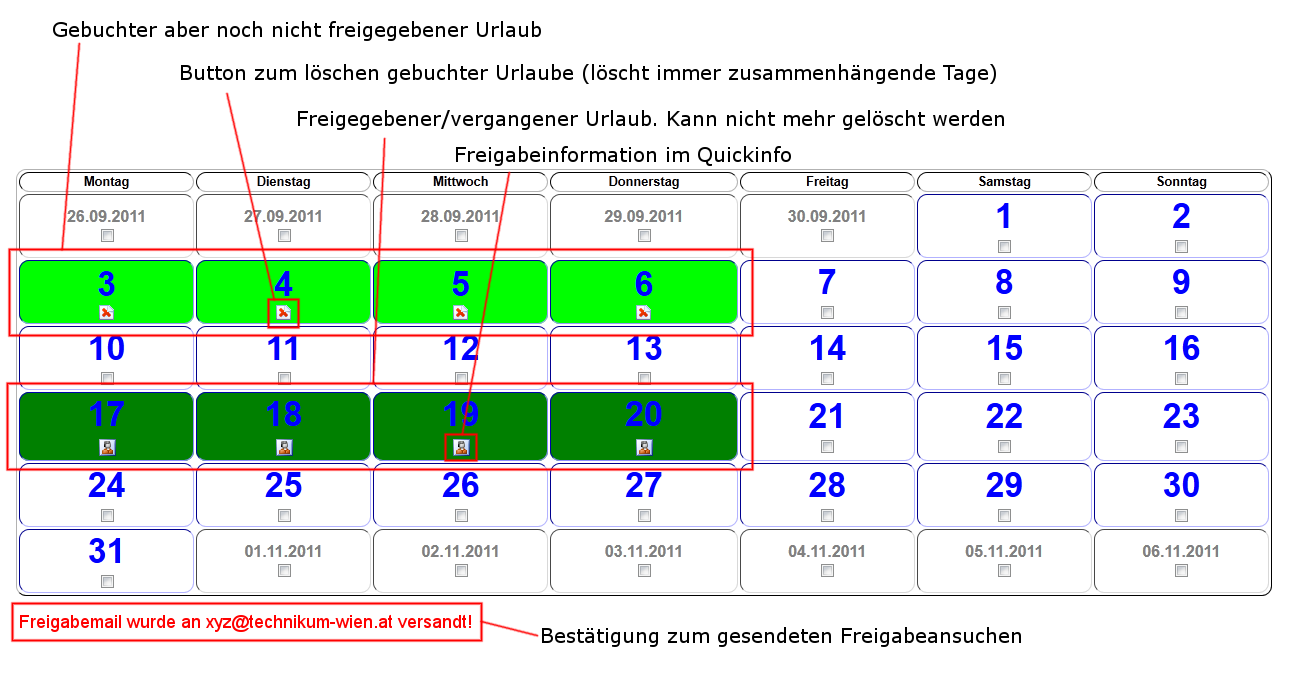
\includegraphics[width=1\textwidth]{CIS_Urlaubstool_Buchungen.png}
	\caption{Booked Vacation }
	\label{CIS_urlaubstool_buchungen}
\end{figure}

\section{Deleting a Booked Vacation}

You can delete a vacation that has been booked but not yet approved by clicking on the x below each vacation day.
Consecutive days are saved as one vacation period and the entire period is deleted again when the delete button is clicked. A click on the delete button in Fig. \ref{CIS_urlaubstool_buchungen}, would therefore delete the entire vacation for August 3rd to the 6th.

{\textit{Please think carefully about your vacation before you book so as not to flood your manager with approval emails and to help avoid any unnecessary confusion.}

\section{Approved Vacation}

After your manager has approved your vacation, it will appear in the vacation tool in dark green and you will no longer be able to delete it.
The delete icon will now be replaced by an information icon. Holding your mouse over this icon will display the infotip where you can see information about who approved your vacation and when.

\achtung{If you book a vacation retroactively for a date in the past (before today's date), it will automatically be marked as approved and you will no longer be able to delete it.}
\chapter{Unavailable Time/Preferred Teaching Time}
\label{zeitsperren_zeitwuensche}

\section{General}

The preferred teaching times and unavailable times can be found under "My CIS".
They primarily serve to support the planning of the teaching schedule to display availability and schedule preferences there.
The vacations booked in the vacation tool (see chapter \ref{urlaubsverwaltung}) are also saved in the system as unavailable times and can as such be edited there as well.

\section{Unavailable Time}
\label{zeitsperren}

In contrast to the preferred teaching time, the unavailable time is intended for marking specific times as unavailable.
An unavailable time is marked with an exact date (from - to) and time (from - to) and can also be provided with additional optional information (e.g. reason for unavailability, substitute,...).

Unavailable time is to be used for example for compensatory time, conferences, sick leave, business travel and other similar events (see Fig. \ref{eingabemaske_zeitsperren}).

\begin{itemize}
	\item Select a "'reason"' for being unavailable from the drop-down menu and enter a meaningful name for the unavailable time.
	\item Please enter the dates and optionally the units for which you will not be available in the "'From"' and "'To"' fields.
	\item Next to "'accessibility"' you can select whether can be reached by telephone, email or if you can not be reached at all while you are away.
	\item Finally, you can also specify someone as your substitute.
	\item Clicking the "'Add"' button confirms and saves your unavailable time.	
\end{itemize}

Selecting "'vacation"' as the reason for your unavailable time is the same as booking a vacation using the vacation tool (see chapter \ref{urlaubsverwaltung}).
For this reason, the unavailable time is processed the same way as booking a vacation, with an email being sent to your manager for approval. Such unavailable times will also be deducted from your accrued vacation.

\achtung{All the days entered will be considered vacation days when calculating your accrued vacation! Therefore, it is necessary to divide longer unavailable times marked as vacation so that they do not include weekends or holidays!}


\begin{figure}
	\centering
	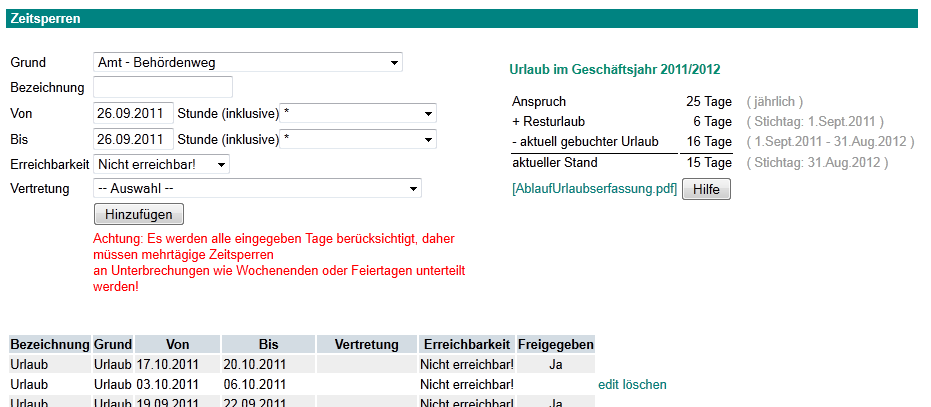
\includegraphics[width=0.70\textwidth]{CIS_Zeitsperre.png}
	\caption{User Interface for Unavailable Times}
	\label{eingabemaske_zeitsperren}
\end{figure}

\subsection{Editing/Deleting Unavailable Times}

The unavailable times you have entered appear in a list below the form.
Next to each entry (excluding approved vacations) you will see an "'Edit"' and a "'Delete"' button which you can use to edit or delete the entry.

You can not edit or delete approved vacations. If you wish to edit or delete an approved vacation, please contact your manager.

\section{Preferred Teaching Time}

The preferred teaching time is entered only once in a static standard weekly grid and is intended to provide a rough template for the availability of the lecturers during a "'normal"' week.

The lecturer can assign values from -2 to +2 for every day and every unit in a week to indicate their availability.
Based on the preferred teaching time, the planning of the teaching schedule can take into account the times a lecturer would like to teach.

The preferred teaching time should and can NOT represent exact availability, but should only serve as a means of orientation.
In order to provide a more detailed overview of availability, please use the unavailable time feature (chapter \ref{zeitsperren}).

\begin{figure}
	\centering
	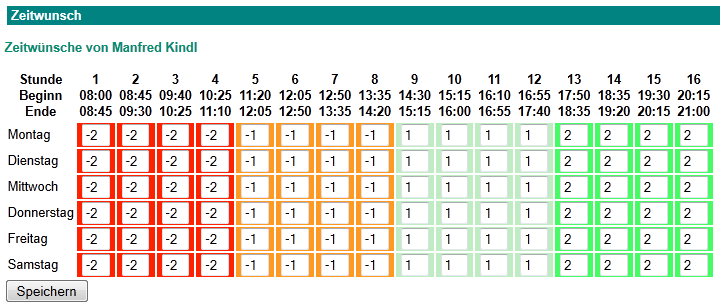
\includegraphics[width=0.70\textwidth]{CIS_Zeitwunsch.png}
	\caption{Preferred Teaching Time Entry Form}
\end{figure}

The default value for the preferred teaching time is "'+1"' for all units.

Now enter the desired value (-2 to +2) in each unit that you want to change and confirm your preferred teaching time by clicking on "'Save"'.

\begin{tabular}{rll}
+2&...&I would like to teach at this time\\
+1&...&I can teach at this time\\
-1&...&I would prefer not to teach at this time\\
-2&...&I can not at all teach at this time\\
\end{tabular}

\idee{You can quickly move between cells by pressing the tab key on your keyboard.}

The values are shown in the background according to a color system (from red to green).
 
Please note the following:

\begin{enumerate}
	\item To make a better optimization possible, please only use the value of -2 if you really can not teach at this time.
	\item The preferred teaching times should be chosen according to the fair play principle, so that at least three times as many teaching units are assigned a positive value as are to be taught according to the teaching assignment. \\ Example: If you are teaching 4 hours/week, then you should select at least 12 hours of preferred teaching times in the grid. 
\end{enumerate}
\chapter{Abgabetool f�r LektorInnen}
\label{Kapitel Aufruf}
Der Aufruf der LektorInnenoberfl�che erfolgt �ber cis.technikum-wien.at/Mein CIS/Bachelor- und Diplomarbeitsabgabe.

\section{�bersichtsliste der Betreuungen}
In der �bersichtsliste (siehe Abbildung \ref{abgabetool_uebersichtsliste}) finden sich alle Betreuungen von Bachelor- und Diplomarbeiten (im FAS unter Projektarbeit als �berbegriff zusammengefasst, daher der Name Projektarbeitsabgabe), deren Autorin oder Autor noch aktiv sind.

\begin {figure}
	\centering
	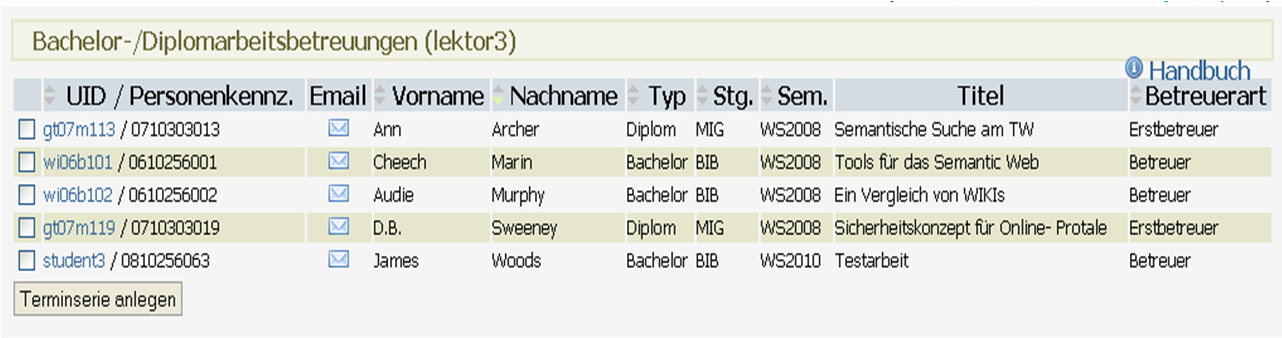
\includegraphics[width=1.0\textwidth]{abgabetool_uebersichtsliste}
	\caption{�bersichtsliste der betreuten Arbeiten}
	\label{abgabetool_uebersichtsliste}
\end {figure}

\subsection{Aufrufen der Termin�bersicht}
Durch Anklicken der UID der Studentin/des Studenten in der zweiten Spalte der �bersichtsliste werden die Termindetails im unteren Teil der Seite angezeigt (Siehe Abbildung \ref{abgabetool_terminverwaltung}).

\subsection{E-Mail an die Studentin/den Studenten}
Durch Anklicken des Briefsymbols in der dritten Spalte wird der E-Mailclient ge�ffnet und die Empf�nger- und Absenderadresse sowie \textit{Bachelorarbeitsbetreuung} bzw. \textit{Diplomarbeitsbetreuung} als Betreff werden vorausgef�llt.

\subsection{Termin f�r mehrere Studentinnen und Studenten ansetzen}
Es gibt auch die M�glichkeit, f�r mehrere Studentinnen und Studenten einen Termin zu setzen. Dazu m�ssen zuerst die betreffenden Zeilen durch Anklicken der Checkbox in der ersten Spalte markiert werden. Danach �ffnet ein Klick auf den Button \textit{Terminserie anlegen} eine Eingabemaske im unteren Teil des Browserfensters. Hier wird dann der Termin eingegeben und durch Dr�cken der Taste \textit{speichern} der Termin f�r alle zuvor markierten Betreuungen gespeichert.

\subsection{Aufruf der Anleitung}
Rechts neben der �berschrift \textit{Bachelor- /Diplomarbeitsbetreuungen} befindet sich ein blauer Icon mit einem weissen i. Durch einfaches Klicken darauf kann diese Anleitung als pdf-Datei aufgerufen werden.

\section{Termin�bersicht}

\begin {figure}
	\centering
	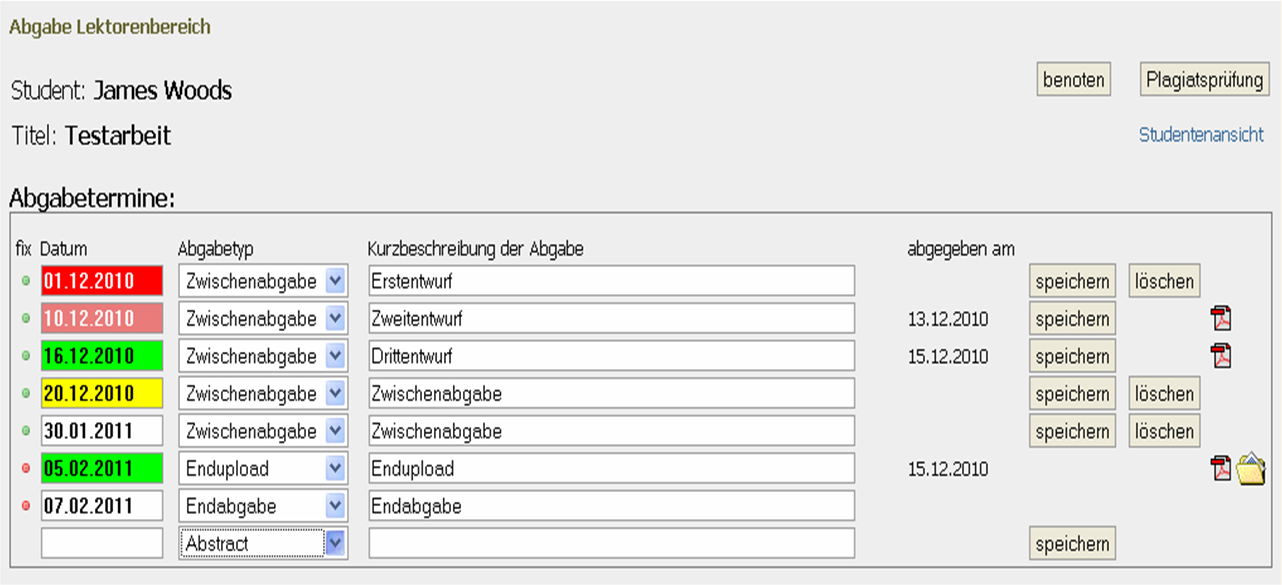
\includegraphics[width=1.0\textwidth]{abgabetool_terminverwaltung}
	\caption{Verwaltung und �bersicht der Termine}
	\label{abgabetool_terminverwaltung}
\end {figure}

\subsection{Termineingabe und -bearbeitung}

\begin{itemize}
	\item Termineingabe: Die unterste Zeile der Liste ist bis auf das Auswahlfeld \textit{Abgabetyp} leer und f�r die Eingabe eines neuen Termins vorgesehen. Geben Sie ein Datum ein, w�hlen Sie den Abgabetyp aus und geben Sie eine kurze Beschreibung der Abgabe ein. Abschlie�end wird mit einem Klick auf den Button \textit{speichern} der Termin eingetragen.
	\item Termin�nderung: Termineintr�ge k�nnen ge�ndert werden, indem Sie die Daten der betreffenden Zeile �ndern und anschlie�end \textit{speichern} dr�cken.
	\item Termin l�schen: Termin k�nnen durch Klicken auf die Taste \textit{l�schen} gel�scht werden. Ist bereits eine Abgabe erfolgt, kann ein Termin nicht mehr gel�scht werden.
	
	\info{�ber alle drei Aktionen wird die Studentin/der Student per Mail informiert}
	\item Die Assistenz kann fixe Termine vergeben, erkennbar an dem roten Bullet unter \textit{fix}. Liegt ein Termin in der Vergangenheit, kann die Studentin/der Student zu diesem nichts mehr hochladen. Soll dennoch etwas hochgeladen werden, mu� die Studentin/der Student bei der Studiengangsassistenz um eine Korrektur des Termins ansuchen.
	
	\info{Es k�nnen nur selbst angelegte Termine ge�ndert und gel�scht werden}
\end{itemize}

\subsection{Farbcode}

\begin{itemize}
	\item wei�:	"normaler" Termin
	\item gelb:	Termin innerhalb der n�chsten 12 Tage
	\item rot:	Termin �berschritten
	\item gr�n:	Abgabe erfolgt
	\item hellrot: Abgabe nach Termin 
\end{itemize}

\subsection{Download der Abgabe und Ansicht der Zusatzdaten}
Durch Klicken auf das Symbol 
\includegraphics{icon_pdf} wird ein Dialogfenster zum Speichern oder Betrachten der Abgabe dieses Termins ge�ffnet.
Bei der Endabgabe m�ssen von der Studentin/dem Studenten zus�tzlich Daten f�r die Publikationsdatenbank eingegeben werden. Diese sollten mittels dem Symbol 
\includegraphics{icon_ordner_endabgabe} vor der Benotung �berpr�ft werden.

\subsection{Benotung}
Rechts oben auf der Temin�bersicht befindet sich der Button \textit{benoten}, mit dem das Formular zur Benotung der Bachelor- bzw. Diplomarbeit aufgerufen werden kann. Die bereits verf�gbaren Daten wie die Daten der Studentin/des Studenten, Titel der Arbeit, Name der Begutachterin/des Begutachters sind bereits vorausgef�llt. Eingetragen m�ssen die verbalen Beschreibungen der Teilbenotungen und die Punkte der Teilbereiche. Aus den Punkten werden nach dem am Formular aufgef�hrten Schl�ssel die Noten sofort mit der Eingabe berechnet. 

Das Formular wird abschlie�end ausgedruckt und unterschrieben bei der Studiengangsassistenz abgegeben.

\subsection{Link zur Plagiatspr�fung}
Neben dem Button f�r das Benotungsformular befindet sich der Aufruf der Internetseite zur Plagiatspr�fung. Dort kann die abgegebene Arbeit hochgeladen werden.

\subsection{Studentenansicht}
Unterhalb des Links zur Plagiatspr�fung wird ein Link f�r die Studentenansicht angezeigt.
Hier wird die Abgabe aus Studentensicht angezeigt. Sie k�nnen von hier aus auch Arbeiten f�r die Studenten hochladen.

\subsection{Termin�bersicht f�r alle Termine}
Unterhalb der Liste der Studierenden gibt es die M�glichkeit, eine Liste mit allen Abgabeterminen der betreuten Studierenden zu erstellen. In dieser Liste werden alle Termine angezeigt die noch in der Zukunft liegen.

\subsection{Alte Arbeiten anzeigen}
Sie k�nnen sich die Termine und Arbeiten der abgeschlossenen Betreuungen einblenden, indem Sie unterhalb der Liste der Studierenden auf den Link "alle betreuten Arbeiten anzeigen" klicken. Es werden dann in der Liste, zus�tzlich zu den normalen Betreuungen, auch die Betreuungen angezeigt die bereits benotet wurden.
\chapter{Abgabetool f�r Studierende}
\label{Kapitel Aufruf}
Der Aufruf der Studierendenoberfl�che erfolgt �ber cis.technikum-wien.at/Mein CIS/Bachelor- und Diplomarbeitsabgabe.

\section{�bersichtsliste der Betreuungen}
In der �bersichtsliste (siehe Abbildung \ref{abgabetool_uebersicht_student}) finden sich alle Betreuungen von Bachelor- und Diplomarbeiten.

\begin {figure}
	\centering
	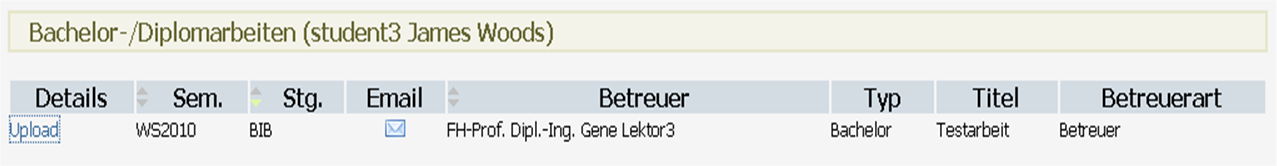
\includegraphics[width=1.0\textwidth]{abgabetool_uebersicht_student}
	\caption{�bersichtsliste der betreuten Arbeiten}
	\label{abgabetool_uebersicht_student}
\end {figure}

\subsection{Aufrufen der Termin�bersicht}
Durch einen Klick auf \textit{Upload} in der ersten Spalte der �bersichtsliste werden die Termindetails im unteren Teil der Seite angezeigt (Siehe Abbildung \ref{abgabetool_termine_student}).

\subsection{E-Mail an den/die Betreuer/Betreuerin}
Durch anklicken des Briefsymbols in der vierten Spalte wird der E-Mailclient ge�ffnet und die Empf�nger- und Absenderadresse sowie \textit{Bachelorarbeitsbetreuung} bzw. \textit{Diplomarbeitsbetreuung} als Betreff werden vorausgef�llt.

\subsection{Aufruf der Anleitung}
Rechts neben der �berschrift \textit{Bachelor- /Diplomarbeitsbetreuungen} befindet sich ein blauer Icon mit einem weissen i. Durch einfaches Klicken darauf kann diese Anleitung als pdf-Datei aufgerufen werden.

\section{Termin�bersicht}

\begin {figure}
	\centering
	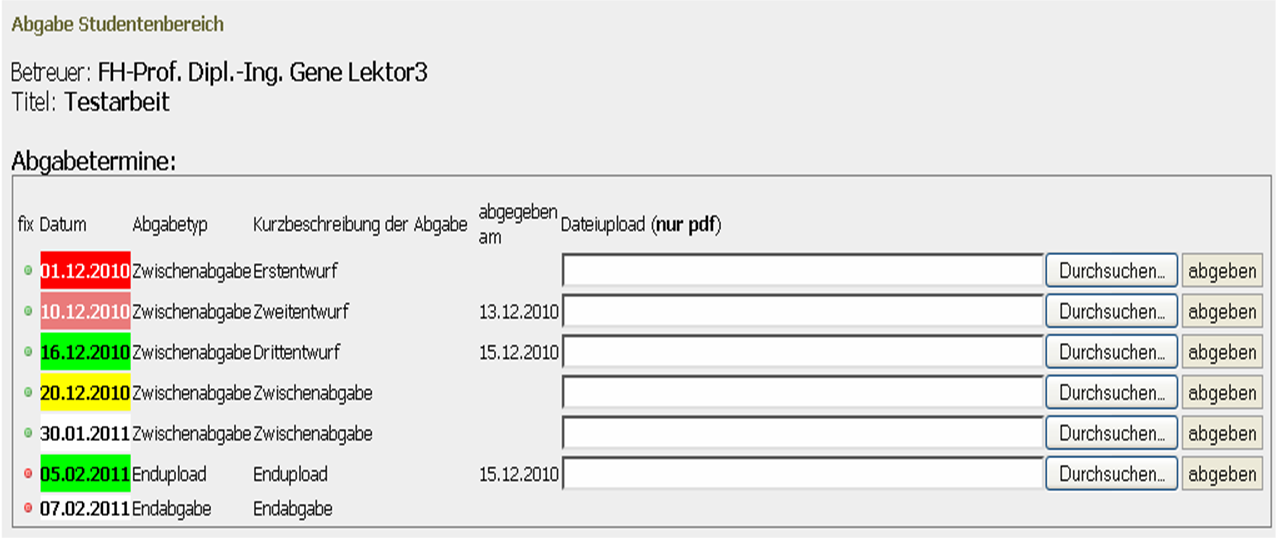
\includegraphics[width=1.0\textwidth]{abgabetool_termine_student}
	\caption{�bersicht der Termine}
	\label{abgabetool_termine_student}
\end {figure}

\subsection{Termine und Dateiupload}

\begin{itemize}
	\item Hier werden Zeilenweise die verschiedenen Termine (Erstentwurf, Zwischenabgabe, Endupload,...) mit einer kurzen Beschreibung angezeigt. 
	\item Die Farbcodierung weist auf den Terminstatus hin (siehe Abschnitt \ref{farbcode})
	\item Klicken Sie beim jeweiligen Termin auf \textit{Durchsuchen} um Ihre Festplatte nach der gew�nschten Datei zu durchsuchen. Klicken Sie danach auf \textit{abgeben} um die Datei wegzuschicken. Ihr/e Betreuer/in wird automatisch per E-Mail �ber die erfolgte Abgabe informiert. Wenn Sie erneut eine Datei hochladen, wird die bestehende Datei �berschrieben.	
	\item Die Studiengangsassistenz kann fixe Termine vergeben, erkennbar an dem roten Bullet in der Spalte \textit{fix}. Liegt ein fixer Termin in der Vergangenheit, k�nnen Sie zu diesem nichts mehr hochladen. Soll dennoch etwas hochgeladen werden, m�ssen Sie bei der Studiengangsassistenz um eine Korrektur des Termins ansuchen.
	
	\info{Es k�nnen derzeit nur Dateien im Format PDF hochgeladen werden}
\end{itemize}

\subsection{Farbcode}
\label{farbcode}

\begin{itemize}
	\item wei�:	"normaler" Termin
	\item gelb:	Termin innerhalb der n�chsten 12 Tage
	\item rot:	Termin �berschritten
	\item gr�n:	Abgabe erfolgt
	\item hellrot: Abgabe nach Termin 
\end{itemize}

\subsection{Zusatzdaten beim Endupload}
Am Termin vom Typ \textit{Endupload} erscheint nach dem Upload ein Formular (siehe Abbildung \ref{abgabetool_zusatzdaten_student}), in dem Sie dazu aufgefordert werden, zus�tzliche Daten f�r die Publikationsdatenbank einzugeben. Diese werden ebenfalls vom Betreuer/der Betreuerin auf Vollst�ndigkeit kontrolliert.
\begin{itemize}
	\item Sprache der Arbeit: Sprache in der die Arbeit verfasst wurde
	\item Kontrollierte Schlagw�rter: Hier k�nnen mit Hilfe eines Schlagwortdienstes, kontrollierte Schlagw�rter hinzugef�gt werden. Siehe Schlagwortdienst
	\item Dt. Schlagw�rter: Schlagw�rter zur Kategorisierung der Arbeit
	\item Engl. Schlagw�rter: Englische Schlagw�rter zur Kategorisierung der Arbeit 
	\item Abstract: Abstract der Arbeit
	\item Abstract engl.: Englischer Abstract der Arbeit
	\item Seitenanzahl: Anzahl der Seiten der Arbeit
	\item Eidesstattliche Erkl�rung: Akzeptieren der Erkl�rung
\end{itemize}
\begin {figure}
	\centering
	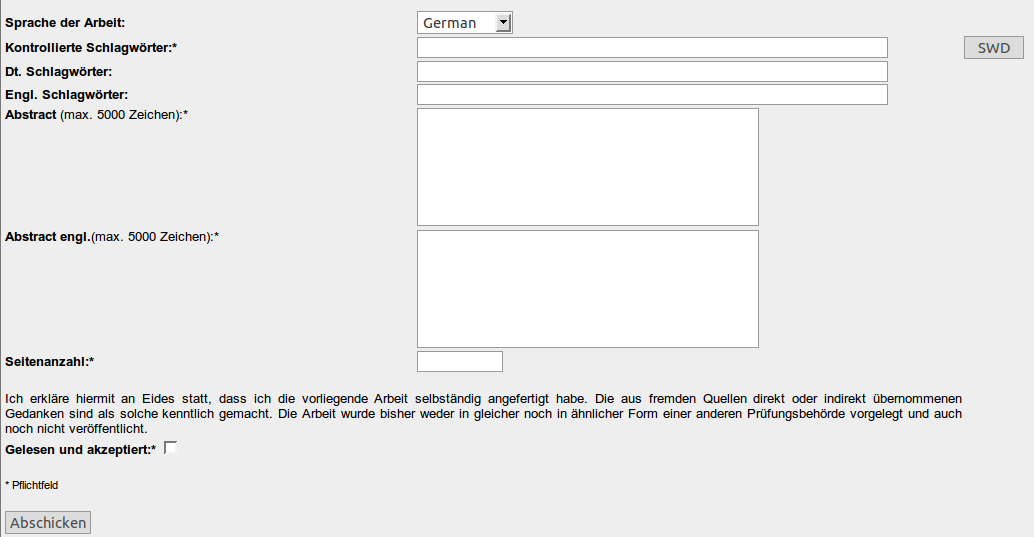
\includegraphics[width=1.0\textwidth]{abgabetool_zusatzdaten_student}
	\caption{Zusatzdaten nach dem Endupload}
	\label{abgabetool_zusatzdaten_student}
\end {figure}

\subsection{Schlagwortdienst}
Kontrollierte Schlagw�rter k�nnen mit Hilfe eines Schlagwortdienstes eingetragen werden.\\
Durch einen klick auf den Button SWD wird der Schlagwortdienst ge�ffnet. 
Sie werden auf eine externe Seite weitergeleitet.
\begin {figure}
	\centering
	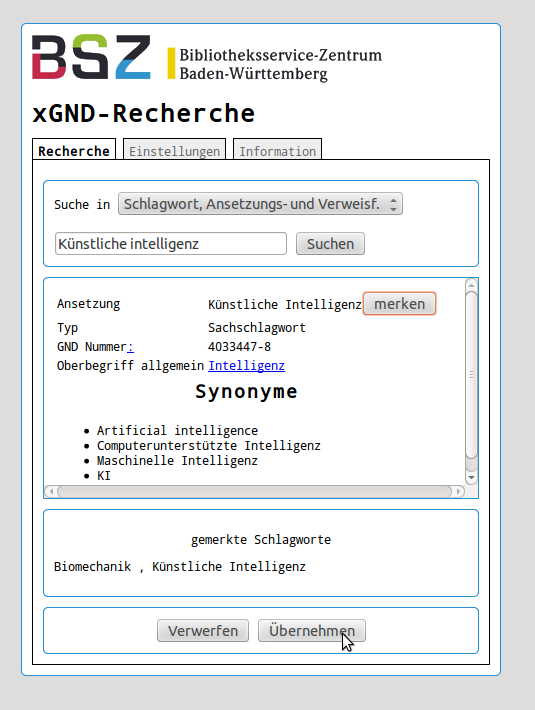
\includegraphics[width=0.5\textwidth]{abgabetool_swd}
	\caption{SWD}
	\label{SWD}
\end {figure}
\\
�ber die Suchfunktion kann nach Schlagw�rtern gesucht werden.
\\Klicken Sie auf den Button ''merken'' um Schlagw�rter auszuw�hlen.
\\Wenn Sie alle Schlagw�rter hinzugef�gt haben k�nnen Sie diese �ber den Button ''�bernehmen'' in das Abgabe-Formular �bertragen.
siehe Abbildung \ref{SWD}

\subsection{Probleme beim Upload}
Falls beim Upload der Datei Probleme auftreten kann dies folgende Gr�nde haben:

\begin{itemize}
	\item Die Dateigr��e darf maximal 15 MB betragen.
	\item Die hochzuladende Datei muss im PDF Format vorliegen. Der Upload von anderen Dateitypen ist nicht m�glich
	\item Deaktivieren Sie eventuell installierte Addons Ihres Browsers (Adblocker, NoScript, etc)
	\item Stellen Sie sicher, dass Javascript aktiviert ist
	\item Versuchen Sie die Arbeit mit einem anderen Browser hochzuladen (zB Firefox)
\end{itemize}
\chapter{Grading tool}

\section{Quickstart}
\label{quickstart}

\subsection{Entering the Final Grade}

The grading tool on the CIS of the Technikum Wien serves as the central tool and interface between the lecturer and the administrative assistant for the grade management.\\

\noindent
{\bf Please use the tool to enter the final grades:}

\begin{enumerate}
\item Select a course under \url{https://cis.technikum-wien.at}-$>$ my CIS-$>$ My LV. Click on the "'Final Grade"' symbol on the overview page, (see Fig. \ref{uebersicht_lv}, page \pageref{uebersicht_lv})
\item Now click on "'Final Grade"' in the upper left corner of the page section.
\item Now enter the grades and accept them with the '-$>$' - button.
(1)
\item Once you have entered all the grades you want to enter at this time (you can return to enter more grades at any time!) you can approve them for the administrative assistant with the "'Approve"' button (in the table header).
(2)\\ 
NOTICE: For reasons of increased security, it is necessary to enter your password when approving grades.\footnote{This refers to your TW password which is used to log into the CIS webpage or the TW computers}
\item Finished!
\end{enumerate}


\begin{figure}[ht]
\begin{center}
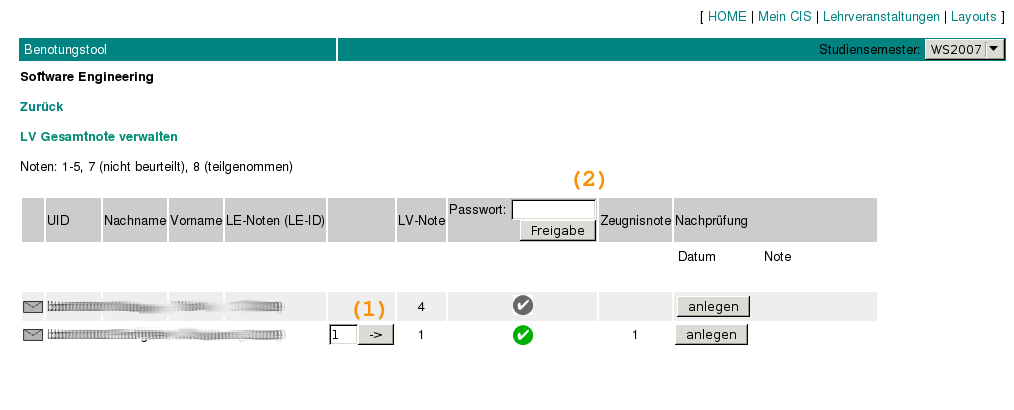
\includegraphics[width=1.0\textwidth]{benotungstool_benotung_lv.png}
\end{center}
\caption{Course Grade}\label{benotung_lv_quick}
\end{figure}

\noindent
For more information, please see chapter \ref{gesamtnote} on page \pageref{gesamtnote}\\

\section{Exercises}
\subsection{Structure}
\noindent
In general, activities are created as follows:
{\em Activities} can be graded directly (e.g. tests).
Alternatively, {\em activities} can also contain unlimited {\em assigments} or {\em checklists}. (However, it is not possible to mix these).
A {\em checklist} may then contain any number of items.
(see the slides in Annex page \pageref{struktur}ff)

\subsection{Creating and Managing Activities}

\begin{figure}[ht]
\begin{center}

\makebox[0pt][l]{
\includegraphics{icon_info}}%
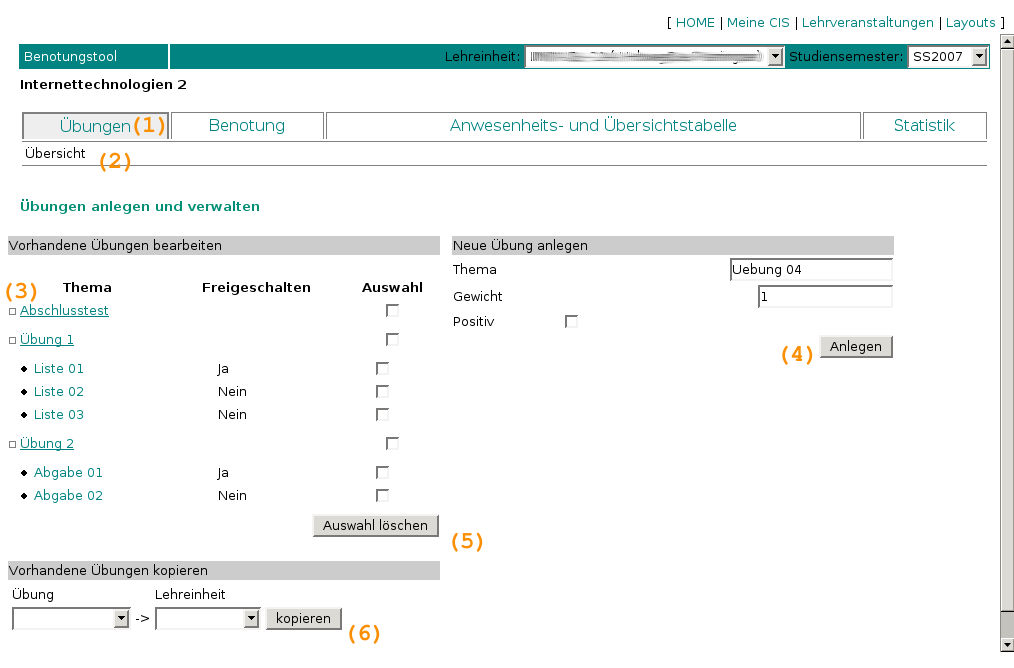
\includegraphics[width=1.0\textwidth]{benotungstool_verwaltung_01.png}

\end{center}
\caption{Activity Management - Overview}\label{verwaltung_01}
\end{figure}

Click on the "'Activities"' tab (see Fig. \ref{verwaltung_01} (1)) - this is also the standard start page.
You can see which level you are currently on within the activity in the subnavigation (2).

The overview page displays all the activities that have been created. 
Clicking the small square in front of the activity name (3) will display all the checklists or assignments in the activity.

Creating a new activity (4): Each activity must be given a name and a point value (for information on how the grades are calculated, see chapter Grading).
If you check the "'Positive"' box, the calculated final grade can only be positive if this activity is completed successfully.

Deleting activities (5): Mark one or more entries to delete them. NOTICE: All the associated data will also be deleted! (sub checklists, assignments, grades already given for the activity, student checklists

Copying activities (6): It is possible to copy an entire activity including all the sub assignments/checklists, as well as all student upload files in other groups of the same course.
Exercises that have been copied once will be synchronized when they are copied again later; i.e. you can adapt an activity in one group and then apply them to the respective activity in another group.\footnote{In future we intend to make it possible to also copy activities from other courses and semesters.}

Clicking on an activity name will open the editing view for the activity. You can edit the activity here, as well as create sub assignments or checklists. It is possible to create either type as long as no other sub elements exist. The first type that you create determines which type can subsequently be used within this activity.

However, once a grade has been given for an activity it will no longer be possible to create any further sub elements. (see chapter \ref{benotung}, page \pageref{benotung}) 

\subsubsection{Assignments}

\begin{figure}[ht]
\begin{center}
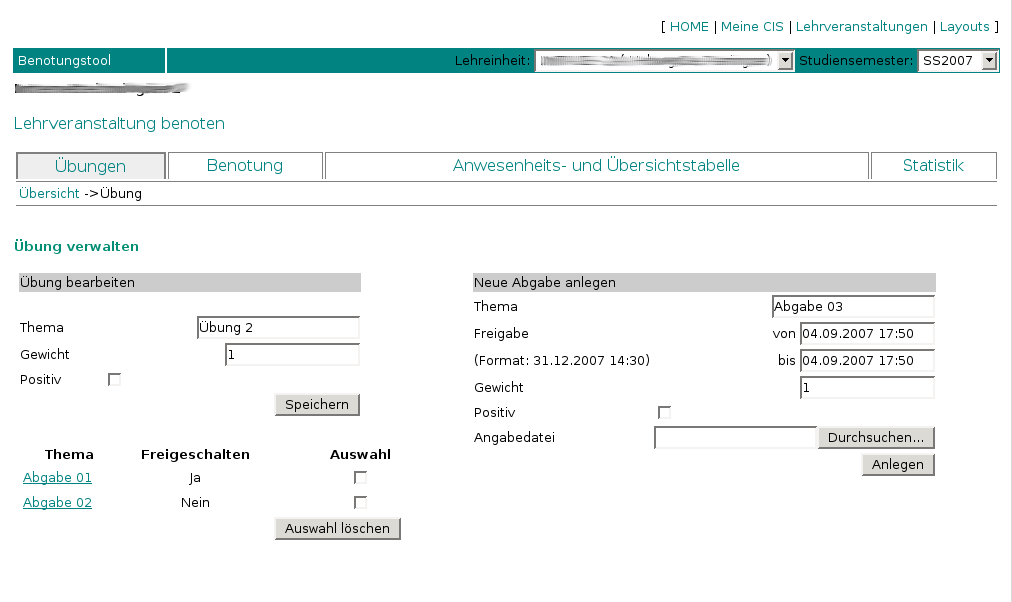
\includegraphics[width=1.0\textwidth]{benotungstool_uebung_detail_abgaben.png}
\end{center}
\caption{Creating Assignments}\label{uebung_detail_abgaben}
\end{figure}

You are in the editing view for an activity (see Fig. \ref{uebung_detail_abgaben}).

To create an assignment you must define the subject, the time by which your student should upload the assignment file, the point value for the assignment within the activity and if it must be completed successfully. In addition, you can also upload an assignment file.\footnote{The file name is automatically generated and assigned to the respective assignment}

Existing assignments can be edited by clicking on the assignment name. (see Fig. \ref{abgabe_detail}). You can change your assignment file here by overwriting it with another assignment or you can delete it by clicking on the [del] link.

\begin{figure}[ht]
\begin{center}
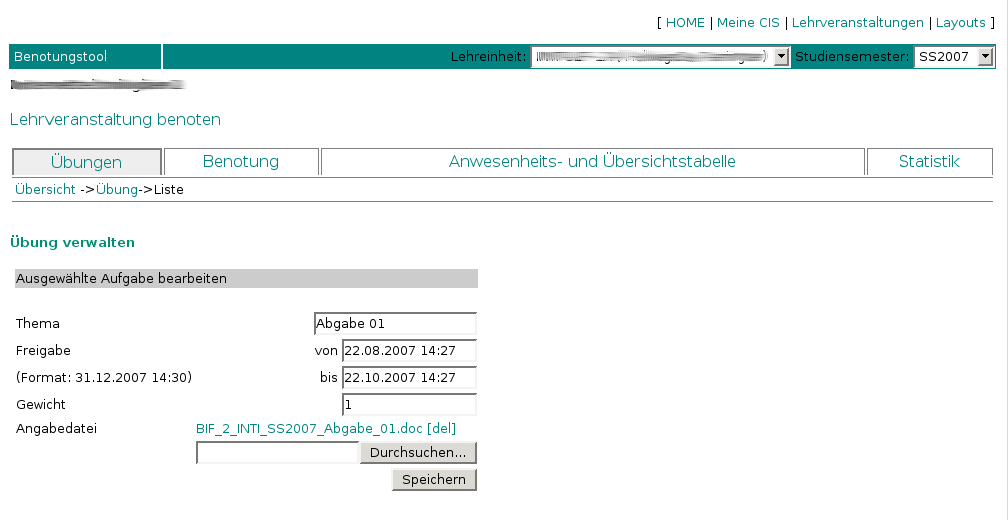
\includegraphics[width=1.0\textwidth]{benotungstool_abgabe_detail.png}
\end{center}
\caption{Editing Assignments}\label{abgabe_detail}
\end{figure}

\subsubsection{Checklists}
\label{kap_kreuzerllisten}

You are in the editing view for an activity (see Fig. \ref{uebung_detail_kreuzerllisten}).

\begin{figure}[ht]
\begin{center}
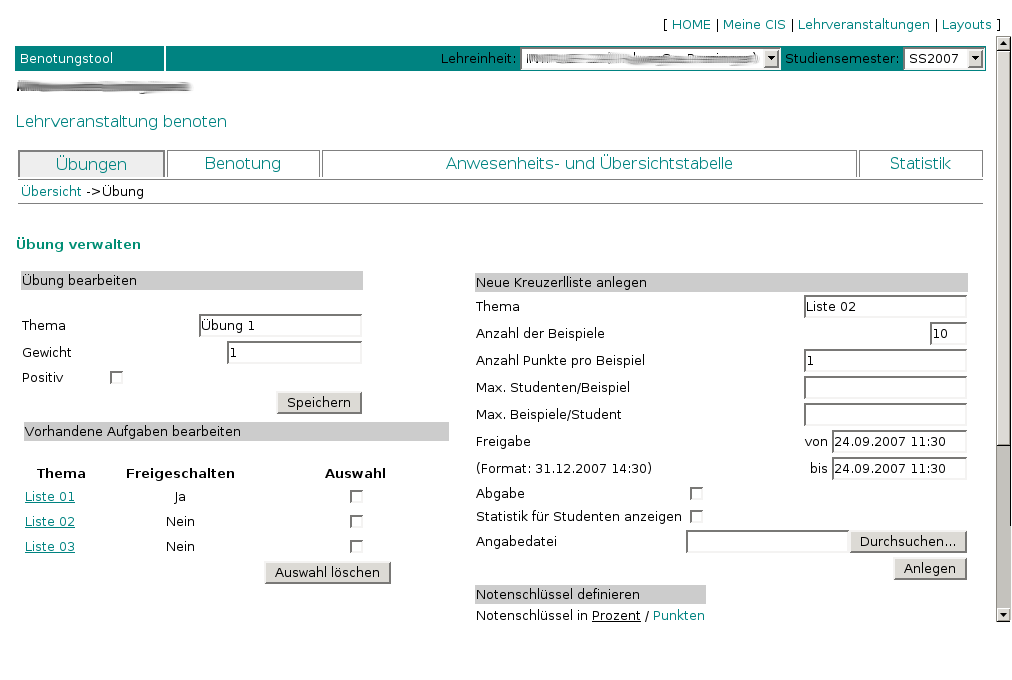
\includegraphics[width=0.9\textwidth]{benotungstool_uebung_detail_kreuzerllisten.png}
\end{center}
\caption{Creating Checklists}\label{uebung_detail_kreuzerllisten}
\end{figure}


To create a checklist you must define the subject, number and point values for the items, the time available for the students to place checkmarks by all the items, as well as whether the statistics for the checkmark distribution should be visible for the students.

If you check the "'Student Uploads"' box, students will be able to upload a file for the checklists. This works the same as an assignment, except that you do not grade these files separately.

In addition, here you can define the maximum number of students who can select a particular item or the maximum number of items that can be selected per student.

Furthermore, you can also upload an assignment file. \footnote{The file name is automatically generated and assigned to the respective checklist}


\begin{figure}[ht]
\begin{center}
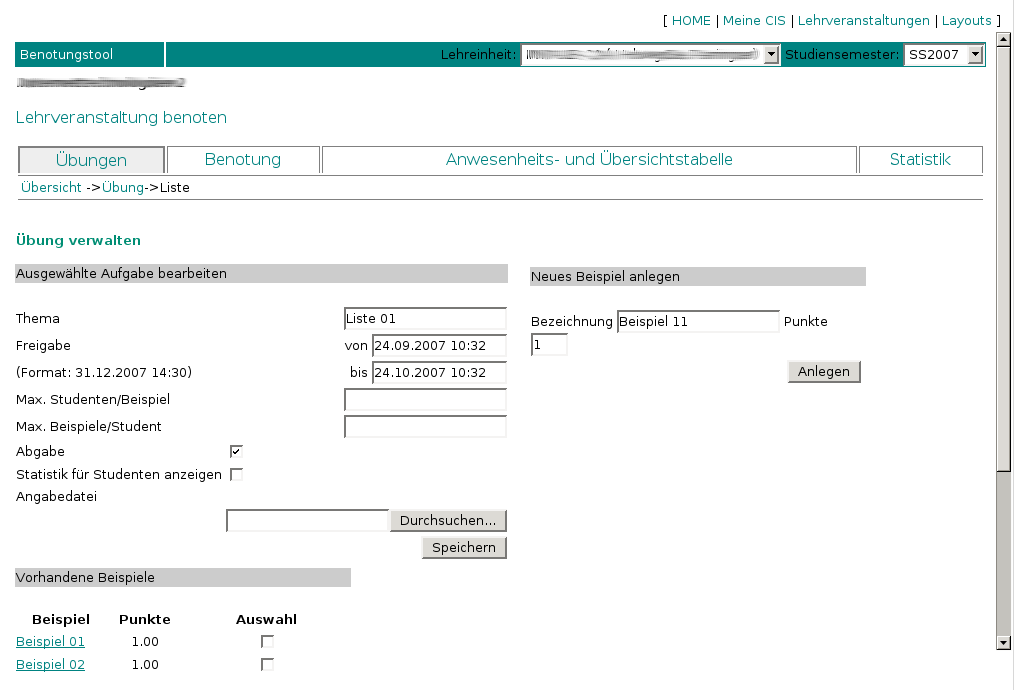
\includegraphics[width=0.9\textwidth]{benotungstool_kreuzerlliste_detail.png}
\end{center}
\caption{Editing Checklists}\label{kreuzerlliste_detail}
\end{figure}

Existing checklists can be edited by clicking on the checklist name. (see Fig. \ref{kreuzerlliste_detail}). You can add, delete or edit items here by clicking on them. You can change your assignment file here by overwriting it with another assignment or you can delete it by clicking on the [del] link.

\subsubsection{Grading Key}
\label{kap_notenschluessel}
The points for all the items for all the checklists within A SINGLE activity are calculated as a grade based on the grading key.
The grading key is defined on the level of the activity that contains the checklists. 

The checklists for this activity will not be included in the automatically calculated grade until a grading key is entered.

You can define the grading key in {\em percentages} or {\em points} (see Fig. \ref{notenschluessel}).

\begin{figure}[ht]
\begin{center}
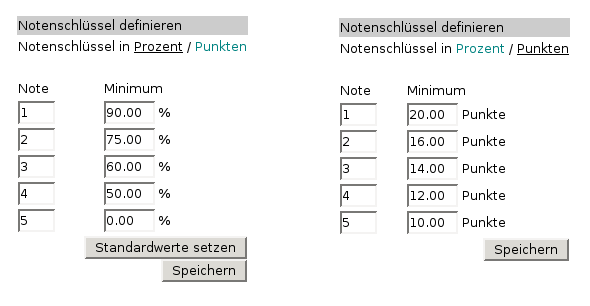
\includegraphics[width=0.8\textwidth]{benotungstool_notenschluessel.png}
\caption{Grading Key in Percentages or Points}\label{notenschluessel}
\end{center}
\end{figure}

You can toggle between the two modes by clicking the respective link. The \underline{underlined mode} is active.

In the {\em percentage} mode you can use the "'Set default values"' button to automatically fill out the fields with the default values.
Adapt the values if necessary, and do not forget to save.

\section{Grading}
\label{benotung}
Click on the Grade tab (see Fig. \ref{benotung_uebungen} (1))

\subsection{Overview and Grading of the Activities}
\label{ben}

\begin{figure}[ht]
\begin{center}
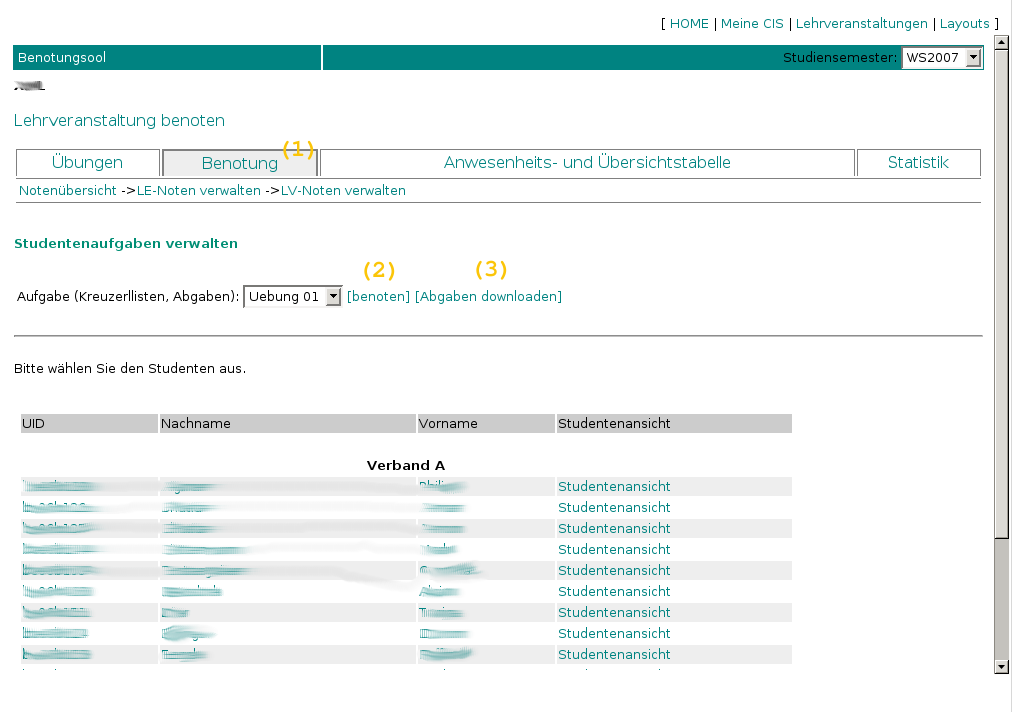
\includegraphics[width=1.0\textwidth]{benotungstool_benotung.png}
\end{center}
\caption{Grading Activities}\label{benotung_uebungen}
\end{figure}

Select an activity, assignment or checklist from the drop-down menu and click "'Grade"' (see Fig. \ref{benotung_uebungen} (2)).
A new page will open with a list of all the students and a grade box or check boxes for the checklist items, as well as the student upload file (see Fig. \ref {notenliste}).
Make your entries and save the page with the button at the bottom right. Close the page.

\begin{figure}[ht]
\begin{center}
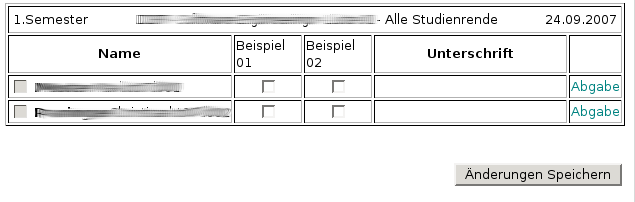
\includegraphics[width=0.7\textwidth]{benotungstool_notenliste.png}
\end{center}
\caption{Grade List}\label{notenliste}
\end{figure}


If there is a student upload for an assignment, a further link will be displayed next to the "'Grade"' link for downloading a ZIP file with all student uploads for this assignment (3).

By clicking on the name of a student, you can assign grades, checklists, participation points and notes for this student in detail. \footnote{The structure is essentially the same as the old "'checklist tool"'}

\subsection{Student View}
\label{studentenansicht}
You can display the student view for the students in your group by clicking on the "'Student View"' link (to the right of the name in the list). A new window will open displaying the student view of the selected student. In this window, you assume the identity of the student and can perform all the same functions there as the student. 

However, this function is only intended for overview/demonstration purposes. Always use the lecturer admin interface as described in section \ref{ben} to make changes to data (add/delete checklists)!

\subsection {Management of Teaching Unit Grades}
\begin{figure}[ht]
\begin{center}
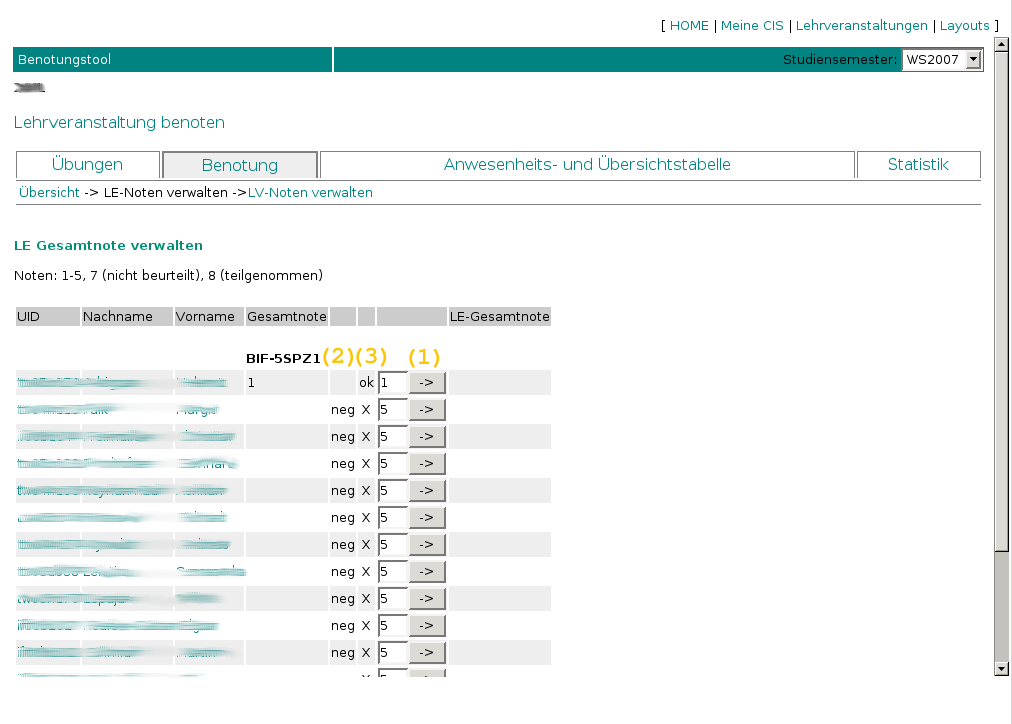
\includegraphics[width=1.0\textwidth]{benotungstool_benotung_le.png}
\end{center}
\caption{Grading Teaching Units}\label{benotung_le}
\end{figure}

A final grade for the teaching unit is calculated based on the grades of the individual activities, assignments and checklists using the point values you defined or the grading key in the case of checklists.
This score is rounded and suggested as the final grade for the teaching unit.
Verify/correct the suggested grades and accept them by clicking the '-$>$' - button.
(see Fig. \ref{benotung_le} (1))

Additional fields:
"'neg"' (2) in the column next to the calculated grade indicates that at least the required, defined positive grade is negative; "'ok"'/"'x"' (3) indicates whether all partial scores are available.

%\input{Final Grade}
%\newpage

\section{Attendance and Overview Table}

This section is still under construction. The current tables are essentially the same as those used in the old "'checklist tool"'.
\section{Final Grade}
\label{gesamtnote}
Select a course under \url{https://cis.technikum-wien.at}-$>$ My CIS-$>$ My LV. Click the "`Final Grade"' symbol on the overview page to open the "`Final Grade"' page.

\subsection{Entering the Final Grade}
\subsubsection{Manually Entering the Final Grade }
\label{ben}

\begin{enumerate}
\item Enter the grade (1) and accept it with the '-$>$' - button.
\item After you have entered all the grades, you can then approve them (see chapter \ref{freigabe} on page \pageref{freigabe}\\).
\end{enumerate}

\begin{figure}[ht]
\begin{center}
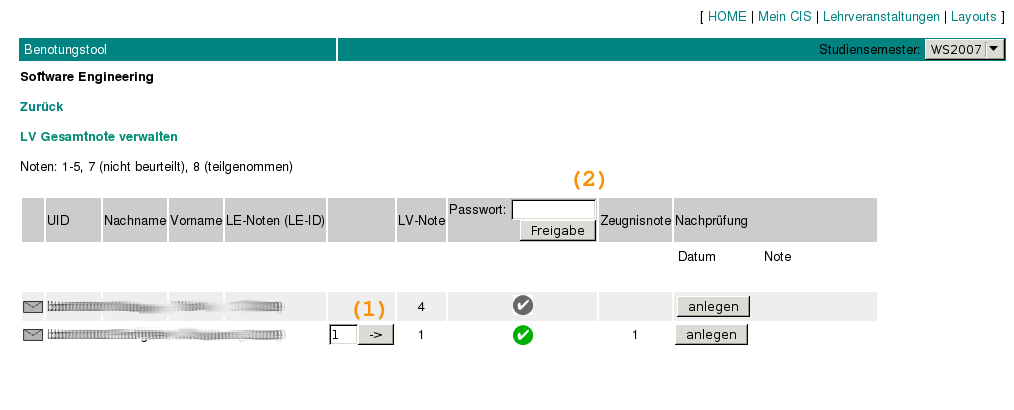
\includegraphics[width=1.0\textwidth]{benotungstool_benotung_lv.png}
\end{center}
\caption{Grading a Course}\label{benotung_lv}
\end{figure}

\subsubsection{Importing Grades from the Activity Tool (Checklist Tool)}
\label{ben}

If an activity has been created and graded in the activity tool (checklist tool) the grade will appear in the final grade.
If the course contains multiple teaching units, the average of all the grades will be suggested as the final grade.

The grade fields are already filled out. Click the '-$>$'- button to accept the grades.

\subsubsection{Importing Grades from Moodle}
\label{ben}

If a Moodle course has been created and graded, the grade will automatically appear in the final grade.
If the course contains multiple Moodle courses, the average of all the grades will be suggested as the final grade.
The grade fields are already filled out. Click the '-$>$'- button to accept the grades.

\subsubsection{Importing Grades from Excel}
\label{ben}

You can also import grades from an Excel file. To do so, use the following steps:

\begin{enumerate}
\item Download the Excel file with the grade list from CIS -$>$ Courses -$>$ Attendance and Grade Lists -$>$ Grade List.
\item Enter the grades in the Excel file.
\item Select the student number and grade columns in Excel for those students for whom you want to import the grades. (no heading)
\begin{figure}[ht]
\begin{center}
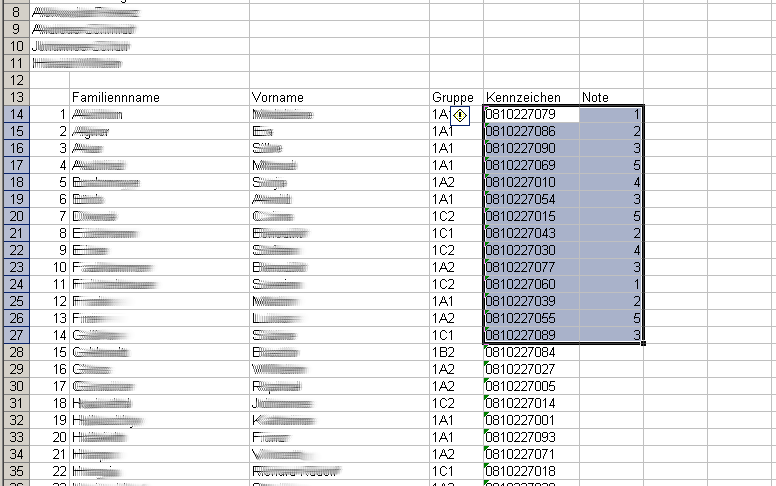
\includegraphics[width=1.0\textwidth]{CIS_Gesamtnote_Excelimport.png}
\end{center}
\caption{Importing from Excel}\label{excelimport}
\end{figure}
\item Copy the marked columns to the clipboard with $<$CTRL$>$+$ <$c$>$ or edit$ >$ copy.
\item Finally, click on the "`Import"' button to import the grades.
\end{enumerate}
\achtung {Existing grades are overwritten without a prompt.}
In order for the grade import to function properly, it is necessary to change some security settings for the browser:

\begin{enumerate}
\item Firefox / Mozilla
	\begin{enumerate}
	\item Open a new browser window.
	\item Enter "`about:config"' in the address bar. 
	(A warning message may appear, which you can skip by single clicking the displayed button)
	\item Search for the entry "`signed.applets.codebase\_principal\_support"'
	\item Change the setting to "`true"' by double clicking it.
	\end{enumerate}
	\achtung {Activating this setting creates a security hole. Therefore, we recommend disabling this setting again after you have finished importing the grades.}
\item InternetExplorer
	\begin{enumerate}
	\item It is not necessary to change any settings when using IE. When you click "Import" a warning message will appear (in IE7) that you will have to confirm by clicking on "`Allow access"'.
	\end{enumerate}
\item Safari, Opera
	\begin{enumerate}
	\item It is NOT POSSIBLE to import grades using the Safari or Opera web browser. Please use Firefox or Internet Explorer.
	\end{enumerate}
\end{enumerate}

\subsection{Approving Grades}
\label{freigabe}

Once you have entered all the grades you want to enter at this time (you can return to enter more grades at any time!) you can approve them for the administrative assistant with the "`Approve"' button (in the table header).
(2)

\info {NOTICE!! For reasons of increased security it is necessary to enter your password when approving grades.\footnote {This refers to your TW password which is used to log into the CIS webpage or the TW computers.}
}

\begin{itemize}
	\item Valid Grades: 1-5, 7 (not graded), 8 (participated)
	\item An information email is sent to you and the administrative assistant for the degree program when the grades are approved. The email includes the student number, first name, last name and grade for the new or edited entries.
	\item Approved entries are marked with a green circle with a check mark.
	\item If you change a grade that has already been approved, it will be marked with a grey circle with a check mark (as a notice for you that the administrative assistant has not yet been informed by email. However, they will still see the new grade immediately in their system interface.)
	\item The administrative assistant can import the approved grade as the transcript grade which will then appear in the next field for your verification.
	\item If the transcript grade differs from the grade you approved, the former is marked with a red border.
\end{itemize}

\subsection{Entering a Resit (2nd Date)}
\label{nachpruefung}

Once you have entered a final grade for a course, a button will appear (after refreshing the page by approving the grades for example) right next to the transcript grade for entering a resit. Once you have entered the resit, a date and grade as well as the "Edit" button will appear (see Fig.\ref{benotung_lv_nachpruefung_quick} (1),(2)).

\begin{figure}[ht]
\begin{center}
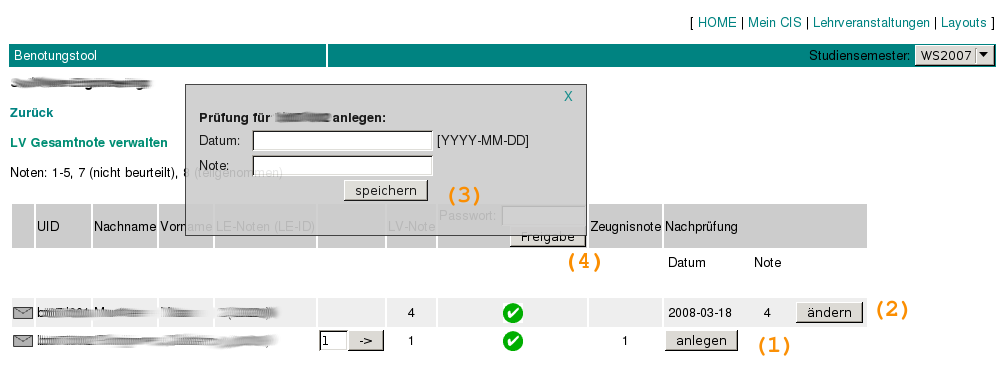
\includegraphics[width=1.0\textwidth]{benotungstool_benotung_lv_nachpruefung.png}
\end{center}
\caption{Final Grade for a Course - Resit}\label{benotung_lv_nachpruefung_quick}
\end{figure}

Click on the respective button to create or edit a resit. Enter the date and grade in the window (3) that appears and then accept the entries by clicking on the "Save" button.

\begin{itemize}
    \item When entering the date, please use the following format: YYYY-MM-DD
    \item Valid grades are once again 1-5, 7 (not graded), 8 (particiapted) and in addition 9 (not yet entered). If you leave the field for the grade blank, then this is interpreted as 9.
    \item After entering a new grade, please do not forget to approve it again by clicking on the the "Approve" button (4).
\end{itemize}

\section{Statistics}

In this section you can view the statistics for the entered checkmarks for the individual checklists just as they are displayed for the students if you have checked the box "'Statistics"' in a checklist.
\section{Annex}

You will find the grading tool here:

\url{https://cis.technikum-wien.at} -$>$ My Cis -$>$ My Course. Click on a course to view its overview page. There you will find the link to the grading tool.
\begin{figure}[ht]
\begin{center}
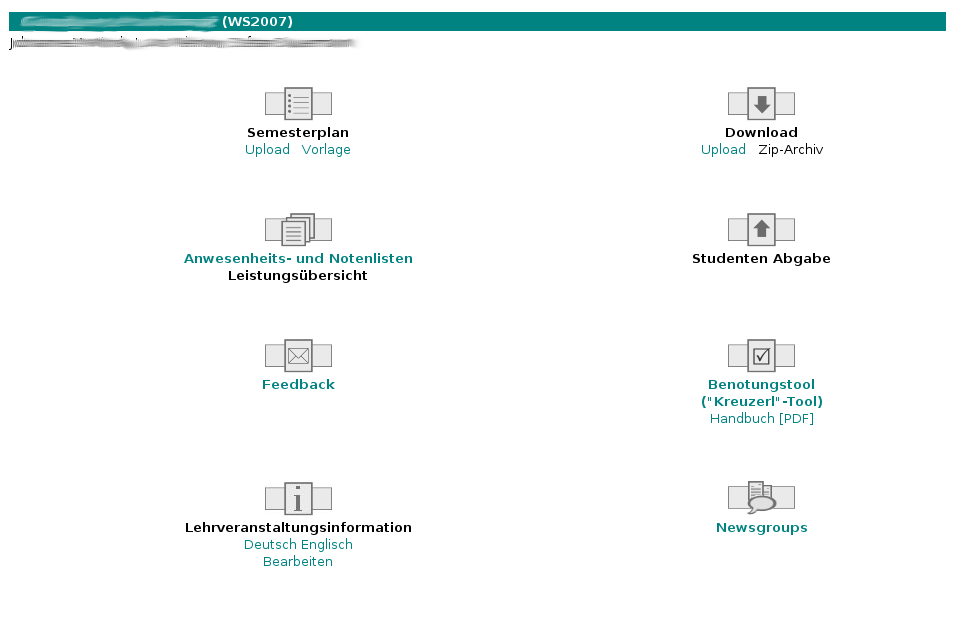
\includegraphics[width=1.0\textwidth]{benotungstool_uebersicht_lv.png}
\end{center}
\caption{Course Overview}\label{uebersicht_lv}
\end{figure}

\begin{figure}[ht]
\begin{center}
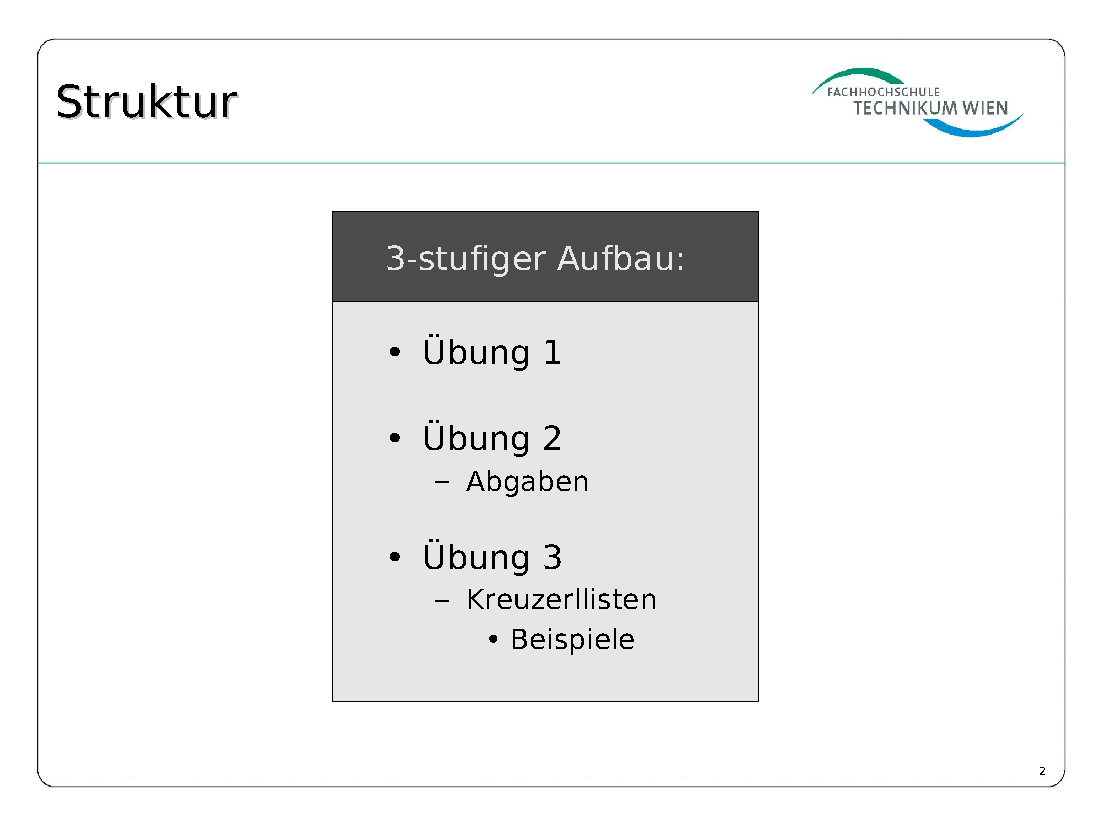
\includegraphics[width=0.9\textwidth]{benotungstool_praes_01.png}
\end{center}
\caption{Presentation: Structure}\label{struktur}
\end{figure}

\begin{figure}[ht]
\begin{center}
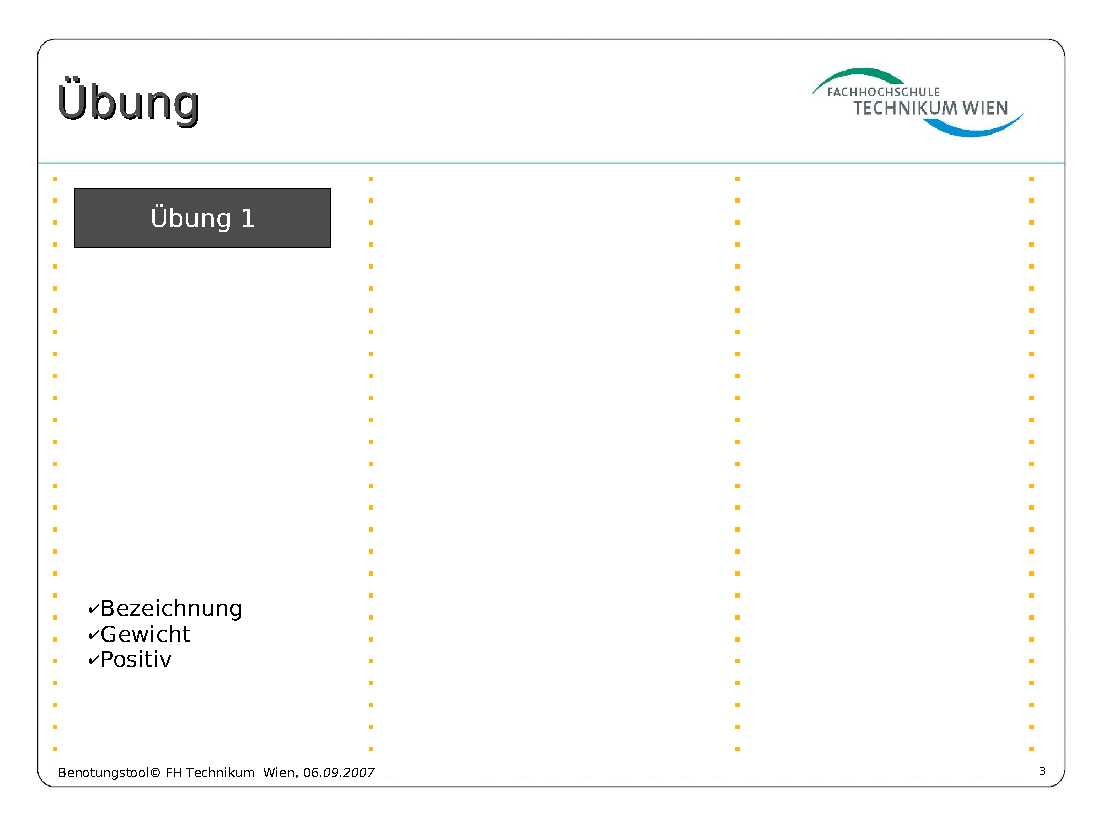
\includegraphics[width=0.9\textwidth]{benotungstool_praes_02.png}
\end{center}
\caption{Presentation: Activity}\label{uebung}
\end{figure}

\begin{figure}[ht]
\begin{center}
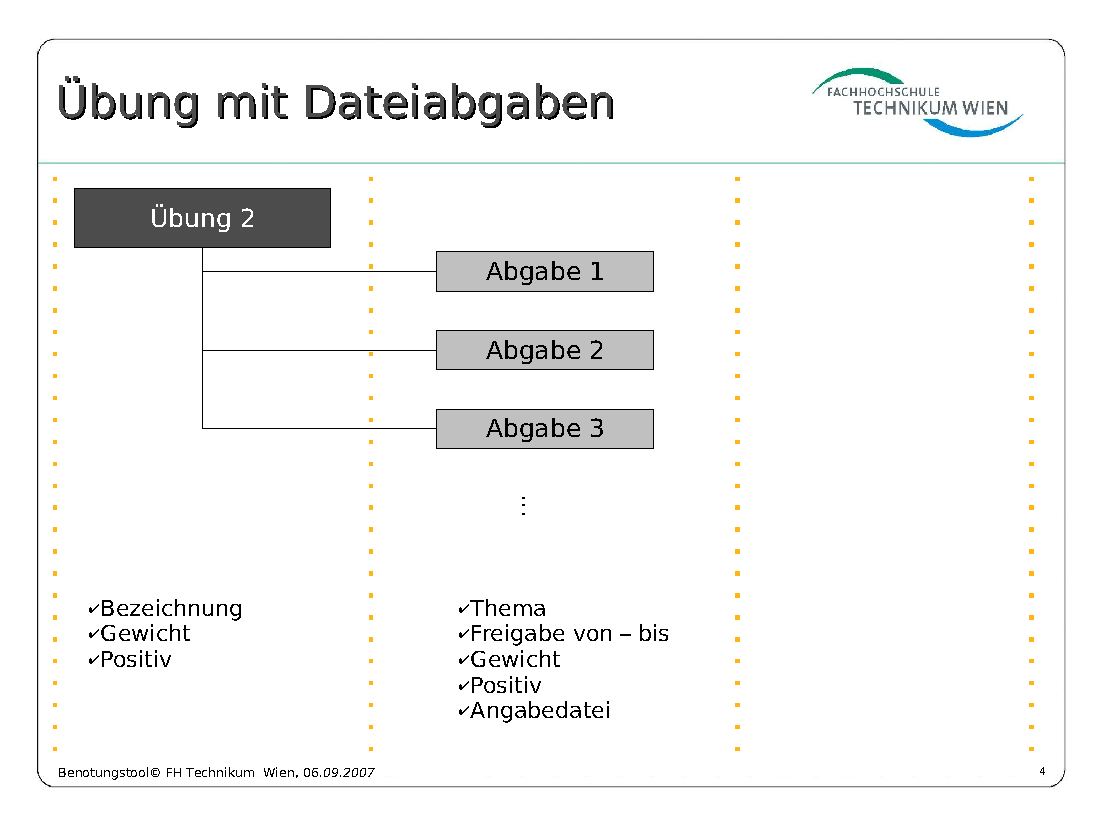
\includegraphics[width=0.9\textwidth]{benotungstool_praes_03.png}
\end{center}
\caption{Presentation: Activity with an Assignment}\label{uebung_abgabe}
\end{figure}

\begin{figure}[ht]
\begin{center}
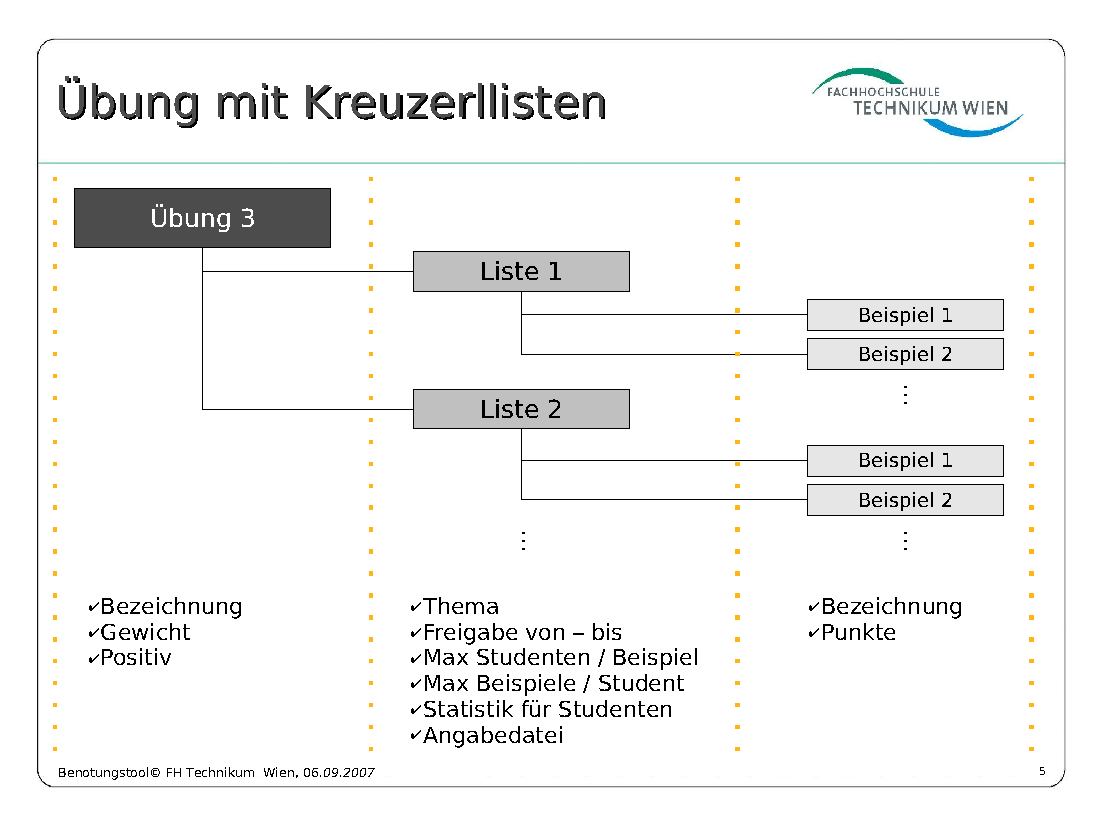
\includegraphics[width=0.9\textwidth]{benotungstool_praes_04.png}
\end{center}
\caption{Presentation: Activity with Checklists}\label{uebung_kreuzerllisten}
\end{figure}

%% Kapitel Ende   %%%%%%%%%%%%%%%%%%%%%%%%%%%%%%%%%%%%%%%%%%%%%%%%%
\appendix							% Beginn des Anhangs
%%\chapter{Schluss}
%\listoftables					% Tabellenverzeichnis
%\listoffigures				% Abbildungsverzeichnis
\end{document}
